% Select document class: 12 point, article
\documentclass[12pt]{article}

\usepackage{makecell}
\usepackage{inputenc}
\usepackage{pdflscape}
\usepackage{longtable}
%\def\includegraphic{}
%\def\includegraphics{}
\usepackage{graphicx}
%\usepackage{xr-hyper}
%\usepackage{xr}
%\usepackage{hyperref}
\usepackage{multirow}
\usepackage{colortbl}
%\usepackage{mathtools}
\usepackage{amsmath}

\def\code#1{\texttt{#1}}
\usepackage{soul}
\newcommand{\red}[1]{\textcolor{red}{#1}}
\newcommand{\blue}[1]{\textcolor{blue}{#1}}

\definecolor{salmon}{rgb}{1,0.4,0}

% AMS = American Mathematical Society; math, symbols, theorems, fonts
\usepackage{amsmath, amssymb, amsthm, amsfonts}

% Enhanced graphics support (https://ctan.org/pkg/graphicx?lang=en)
\usepackage{graphicx}

% Set default graphics path (replace 'figures/' with whatever directory your images are in)
%\graphicspath{{figures/}}
 
% Control layout of itemize, enumerate, description (https://ctan.org/pkg/enumitem?lang=en)
\usepackage{enumitem}

% Header and footer formatting options
\usepackage{fancyhdr}

% Control float placement. [section] = "stop floats at section boundaries is to change the definition of “\section” to include “\FloatBarrier”"
\usepackage[section]{placeins}

% Hypertext (links) in LaTeX. [option] = remove color and border on links.
\usepackage[hidelinks]{hyperref}

%\usepackage[all]{xy}
%\usepackage{mathtools}

% Programming facilities for LaTeX class and package authors
\usepackage{etoolbox}

% Indent first paragraph of every 'chapter' aka section
\usepackage{indentfirst}

% Title formatting option. [explicit] = make titles all caps
\usepackage[explicit]{titlesec}

% Standard package for selecting font encodings. [T1] = Support for accented characters
\usepackage[T1]{fontenc}

% Charter fonts
\usepackage{charter}

%\usepackage[expert]{mathdesign}

% Control table of contents, figures, etc
\usepackage{tocloft}

% Set space between lines. [option] = Double/single spacing necessary for properly formatting ToC/LoFT and titles.
\usepackage[doublespacing]{setspace}

% Create normal/logarithmic plots in two and three dimensions
\usepackage{pgfplots}
% Request a specific version
\pgfplotsset{compat=1.5}

\newcommand\scalemath[2]{\scalebox{#1}{\mbox{\ensuremath{\displaystyle #2}}}}

% Modify section headers (aka chapters) to be: centered, single space, large, bold, preceded with the word 'CHAPTER 'and with 0.4 em of space before title 
\titleformat{\section}[block]{\centering\singlespace\large\bf}{CHAPTER \thesection \hspace{0.4em} \MakeUppercase{#1}}{0em}{}{}

% Modify unnumbered section headers (aka chapters) to be: centered, single space, large, bold, preceded with the word 'CHAPTER 'and with 0.4 em of space before title 
%   We use unnumbered section headers for Acknowledgements, Dedication, Bio, etc. for consistency
\titleformat{name=\section,numberless}[block]{\centering\singlespace\large\bf}{\hspace{0.4em} \MakeUppercase{#1}}{0em}{}{}

% Remove spacing left of, above, and below sections and subsections
%\titlespacing{command}{left spacing}{before spacing}{after spacing}[right]
\titlespacing{\section}{0pt}{0pt}{0pt}
\titlespacing{\subsection}{0pt}{0pt}{0pt}
\titlespacing{\subsubsection}{0pt}{0pt}{0pt}

% Modify TOC entries with tocloft: insert the word 'Chapter ' and then add 6em of space after the word
\renewcommand{\cftsecleader}{\cftdotfill{\cftdotsep}}
\renewcommand{\cftsecpresnum}{Chapter }
\cftsetindents{section}{0em}{6em}

% Call the other parts of the document 'part' and make the table of contents print them correctly
\renewcommand{\cftpartfont}{}
\renewcommand{\cftpartpagefont}{}
\renewcommand{\cftpartleader}{\cftdotfill{\cftdotsep}}
\renewcommand{\cftbeforepartskip}{0em}
\renewcommand{\cftpartindent}{1.5em}

% Change spacing above chapters in toc, remembering that they are really sections
\setlength{\cftbeforesecskip}{0em}

% Adds space after ToC entries to make them appear double-spaced
\renewcommand\cftsecafterpnum{\vskip\baselineskip}
\renewcommand\cftsubsecafterpnum{\vskip\baselineskip}
\renewcommand\cftsubsubsecafterpnum{\vskip\baselineskip}
\renewcommand\cftpartafterpnum{\vskip\baselineskip}

% Add space after LoF entries to make them appear double-spaced
\renewcommand\cftfigafterpnum{\vskip\baselineskip}

% Add space after LoT entries to make them appear double-spaced
\renewcommand\cfttabafterpnum{\vskip\baselineskip}

% Remove extra space above and below theorems, lemmas, props, etc. The important point in the following is: 0pt preskip and 0pt postskip
\makeatletter
\def\thm@space@setup{\thm@preskip=0pt
\thm@postskip=0pt}
\makeatother
\newtheoremstyle{newstyle}      
{} % Aboveskip 
{} % Below skip
{\mdseries} % Body font e.g.\mdseries,\bfseries,\scshape,\itshape
{} % Indent
{\bfseries}  % Head font e.g.\bfseries,\scshape,\itshape
{.} % Punctuation afer theorem header
{ } % Space after theorem header
{} % Heading

% The above does not fix the spacing around proof environments; use the following to fix: The crucial point is "topsep0\p@", i.e., topsep = 0 pt. The rest is essentially copied from the standard AMS environment.
\makeatletter
\renewenvironment{proof}[1][\proofname]{\par
  \pushQED{\qed}%
  \normalfont \topsep0\p@\relax
  \trivlist
  \item[\hskip\labelsep\itshape
  #1\@addpunct{.}]\ignorespaces 
}{
  \popQED\endtrivlist\@endpefalse
}
\makeatother

% Remove default "References" text from \bibliography call
%   Removing this code will cause "References" to appear twice in the bibliography: once for the \thebibliography call and once for the \section*{References} call
\patchcmd{\thebibliography}{\section*{\refname}}{}{}{}

% Remove spacing between bibliography entries
% Set "OLDthebibliography" to be "thebibliography"
\let\OLDthebibliography\thebibliography
% Renew command with 0pt spacing for paragraph and item separation
\renewcommand\thebibliography[1]{
    \OLDthebibliography{#1}
    \setlength{\parskip}{0pt}
    \setlength{\itemsep}{0pt plus 0.3ex}
}

% Formatting
\usepackage[left=1in,right=1in, top=1in, bottom=1in]{geometry}
% \arraystretch = the FACTOR for spacing between two rows (Default = 1) 
\renewcommand{\arraystretch}{0.85}
% \baselinestretch = The spacing between lines in a document (used for "double spacing")
\renewcommand{\baselinestretch}{2}
% \headrulewidth = "The thickness of a line under the header and above the footer"
\renewcommand{\headrulewidth}{0pt}

% Define the StarTeX mathematical symbol
\newcommand{\Mdef}[2]{\newcommand{#1}{\relax \ifmmode #2 \else $#2$\fi}}

% Spacing commands, which may or may not be used in the following.
\newcommand{\one}{{\rm \bf1}\hspace*{-0.035in} {\rm l}}
\newcommand{\nd}{\noindent}
\def\para#1{\vskip 0.4\baselineskip\noindent{\bf #1}}
\newcommand{\Vspc}{\vspace*{0.1in}}

\newcommand{\ID}{\index}
\makeatletter \@addtoreset{equation}{section} \makeatother

% Section Labeling
\renewcommand{\thesection}{\arabic{section}}

% Equation Numbering Ex. Section 3, Equation 2 = Equation 3.2
\renewcommand{\theequation}{\thesection.\arabic{equation}}

\renewcommand{\cftsecfont}{}
\renewcommand{\cftsecpagefont}{}

% List of Tables edits
\renewcommand{\cfttabpresnum}{Table }
\renewcommand{\cfttabindent}{1.0em}
\renewcommand{\cfttabnumwidth}{5.0em}

% List of Figures edits
\renewcommand{\cftfigpresnum}{Figure }
\renewcommand{\cftfigindent}{1.0em}
\renewcommand{\cftfignumwidth}{5.5em}

% Start document
\begin{document}

% Compile the title and jump to new page
% Create title (centered and bold font)
\centerline{\uppercase{\bf Disease understanding and drug repurposing}}
\vspace{-0.4cm}
\centerline{\uppercase{\bf through pathway analysis}}
%\vspace{-0.4cm}
%\centerline{\bf TITLE LINE 3 (if needed)}

\vskip-0.4cm
\thispagestyle{empty}

% Center the following text:
\begin{center}
    \vspace{-0.4cm}
    by \\
    {\bf \uppercase{Tuan Minh Nguyen}}\\ % Full Name
    {\bf \uppercase{Dissertation}}\\  % THESIS (MS Thesis) or DISSERTATION (Ph.D Dissertation)
    Submitted to the Graduate School,\\
    of Wayne State University,\\
    Detroit, Michigan\\
    in partial fulfillment of the requirements\\
    for the degree of\\
    {\bf DOCTOR OF PHILOSOPHY} % MASTER OF SCIENCE / MASTER OF ARTS / DOCTOR OF EDUCATION / DOCTOR OF PHILOSOPHY / etc.
\end{center}

% Left-align the following text:
\begin{flushleft}
    \vspace*{-0.20in}
    \hspace*{3.09in}2025 % Use the year you will graduate
    \hspace*{3.09in}MAJOR: COMPUTER SCIENCE\\ % Major here
    \hspace*{3.09in}Approved By:\\
     \vspace{1cm}
     \hspace*{3.09in}---------------------------------------------------\\
    \vspace*{-0.25in}
    \hspace*{3.09in}Dr. Sorin Draghici\hspace*{1in} Date\hspace*{0.1in}\\
       \vspace{1cm}
    \vspace*{-0.25in}
         \hspace*{3.09in}---------------------------------------------------\\
            \vspace{1cm}
             \vspace*{-0.25in}
         \hspace*{3.09in}---------------------------------------------------\\
            \vspace{1cm}
             \vspace*{-0.25in}
         \hspace*{3.09in}---------------------------------------------------\\
         
    % Add these lines below for the cover that will be signed by advisors
    % WSU Graduate School asked that these lines below be removed for publiction
    %   Ex. When printing copies for dissertation committee, UNCOMMENT THE LINES BELOW.
    %   Ex. When sending a PDF of the thesis to WSU Grad school for format check (through ETD), COMMENT THE LINES BELOW. 
    %\bigskip
    %\hspace*{3.09in}-----------------------------------------------------------\\
    %\medskip
    %\hspace*{3.09in}-----------------------------------------------------------\\
    %\medskip
    %\hspace*{3.09in}-----------------------------------------------------------\\
    %\medskip
    %\hspace*{3.09in}-----------------------------------------------------------
\end{flushleft}

\newpage

% Begin roman numbering starting with page 2
%   WSU formatting requires: No pg number on title, pg numbering begins with page 2, pg numbering begins in roman numerals
\pagestyle{fancy} \chead{} \rhead{} \lhead{}
\pagenumbering{roman} \lfoot{}\cfoot{\thepage}\rfoot{}
\setcounter{page}{2}

%% Compile dedication page
%\phantomsection
%% Use unnumbered section for dedication
\section*{DEDICATION}

% Add reference to the table of contents {toc} at the section level {section} titled "Dedication" {Dedication}
\addcontentsline{toc}{section}{Dedication}
\begin{center}
To my parents with their unlimited support, \\my wife for her dedication to the family,\\ and my son for his smile. \end{center}

%\newpage
%
%% Compile acknowledgements page
%\phantomsection
%% Use unnumbered section for acknowledgements
\section*{ACKNOWLEDGEMENTS}

% Add reference to the table of contents {toc} at the section level {section} titled "Acknowledgements" {Acknowledgements}
\addcontentsline{toc}{section}{Acknowledgements}

	I would like to express my deepest gratitude to my supervisor, Dr. Sorin Dr\u{a}ghici, for his invaluable guidance, continuous support, and encouragement throughout my research journey. His insightful feedback and unwavering patience has been instrumental in shaping this dissertation and my growth as a researcher.

I am also profoundly grateful to my parents for their unconditional love, support, and sacrifices that have made this journey possible. Their belief in me has been a constant source of motivation.

To my wife, Truc Bui, your patience, understanding, and unwavering support have been my greatest strength. Your encouragement has kept me going through the challenges of this journey, and for that, I am forever thankful.

I would also like to extend my appreciation to my current and former lab mates, especially Tin Nguyen, Adib Shafi, Douglas Craig, Cristina Mitrea and Radu Vanciu, whose collaboration, insightful discussions, and camaraderie have made this experience both enriching and enjoyable. Their support and shared knowledge have greatly contributed to this work.

Finally, I acknowledge everyone who has contributed, directly or indirectly, to the completion of this dissertation. Your support and encouragement have meant the world to me.

%Thank you.



%\newpage

% Enter single spacing environment for toc, lot, and lof (see below)
\begin{singlespace}

% Create Table of Contents (toc)
\renewcommand{\contentsname}{\hfill\large TABLE OF CONTENTS \hfill}
\tableofcontents
\newpage

% Create List of Tables (lot)
\phantomsection
\addcontentsline{toc}{section}{List of Tables}
% Add lot to toc
\renewcommand{\listtablename}{\hfill\large LIST OF TABLES \hfill}
\listoftables
\newpage

% Create List of Figures (lof)
\phantomsection
\addcontentsline{toc}{section}{List of Figures}
% Add lof to toc
\renewcommand{\listfigurename}{\hfill\large LIST OF FIGURES \hfill}
\listoffigures

% Exit single spacing environment for remaining contents
\end{singlespace}

\clearpage

% Begin arabic page numbering
%   WSU formatting requires: content page numbering is arabic
\pagestyle{fancy} \chead{\thepage} \rhead{} \lhead{}
\pagenumbering{arabic} \lfoot{}\cfoot{}\rfoot{}
\setcounter{equation}{0}

\section{Introduction}
\label{chap:Introduction}


Many life science experiments focus on comparisons between two phenotypes such as disease vs. control, treated vs. not treated, drug A vs. drug B, etc. Microarrays and more recently, RNASeq assays, allow researchers to measure all genes and subsequently  yield a list of differentially expressed (DE) genes. The challenge is to translate these measurements and lists of DE genes into a better understanding of the underlying biological phenomena, and in particular an understanding of its mechanisms. Analysis approaches such as pathway analysis~\cite{DraghiciOntologicalToolsReview:2005,Khatri:2012, mitrea2013methods, tarca2013comparison, nguyen2018network, ihnatova2018critical, nguyen2019identifying}, network analysis~\cite{mitra2013integrative} and gene ontology (GO) analysis~\cite{DraghiciOntologicalToolsReview:2005,Rhee:2008}, have been very successful in the past two decades in helping to translate such lists of DE genes into meaningful insights of the underlying biological phenomena. 

Pathway databases such as Kyoto Encyclopedia of Genes and Genomes (KEGG)~\cite{Kanehisa:2000}, Reactome~\cite{croft2014reactome}, BioCarta~\cite{BioCartaWWW}, NCI-PID ~\cite{Schaefer:2009}, WikiPathways~\cite{pico2008wikipathways}, and PANTHER~\cite{thomas2003panther} model signaling pathways as networks in which nodes represent related genes or gene products and edges symbolize interactions among them based on prior knowledge. 
Pathway analysis approaches use available pathway databases and the given gene expression data to identify the pathways which are significantly impacted in a given condition. 
Because of the importance of this type of analysis, more than hundreds of pathway analysis methods have been proposed thus far~\cite{DraghiciOntologicalToolsReview:2005,Khatri:2002,mitrea2013methods}.
It would now become a challenge for any researcher to choose which pathway analysis method is the most suitable for their analysis. 
Although there have been some review studies before, all of them have some limitations.

Here, for the first time, we present a comparison of the performances of 13 representative pathways analysis methods on \red{97} real data sets from two species: human and mouse. 
To our knowledge, this is the highest number of real data sets used in a comparative study on pathway analysis methods.
The second assessment investigates the potential bias of each method and pathway.

This article provides precise, objective, and reproducible answers to the following important and currently unanswered questions: (i) is there any difference in performance between non-TB and TB methods?, (ii) is there a method that is consistently better than the others in terms of its ability to identify target pathways, accuracy, sensitivity, specificity, and the Area Under the receiver operating characteristic Curve (AUC)?, (iii) are there any specific pathways that are biased (in the sense of being more likely or less likely to be significant across all methods)?, and (iv) do specific methods have a bias toward specific pathways (e.g. is pathway X likely to be always reported as significant by method Y)?. 
This article provides a guidance to help researchers select the right method to deploy in analyzing their data based on any kind of scientific criteria. 
At the same time, this article will be of interest to any computational biologists or bioinformaticians involved in developing new analysis methods. 
For such researchers, this article is expected to become the benchmark against which any future analysis method will have to be compared. 
Finally, because of the bias analysis of all known KEGG pathways included here, this article is also expected to be extremely useful to many people involved in the curation and creation of pathway databases.

A particular sub-problem in this area focuses on the identification of upstream regulators that may explain the observed changes. In principle, such upstream regulators could be of different types including: genes (e.g. gene encoding transcription factors), miRNA, drugs, chemicals, or toxicants. This type of analysis is generally referred to as ``causal analysis''~\cite{schadt:2005, chindelevitch2012causal, kramer2013causal, felciano2013predictive}. 


Some diseases are caused by exposing to harmful or toxic environment, such as wild fire smoke or polluted water sources. These toxicants can be either a product of human activities or from natural disasters. In these cases, the presence of a chemical substance  is responsible for the changes in  the gene expression profiles and  therefore, for creating the phenotypes. 
In other situations,  a phenotype and its associated  gene expression changes  can be caused by the lack of a necessary chemical  that plays an important metabolic role, e.g. iodine deficiency. 
Identifying the chemical, drug, or toxicant (CDT) that perturbs the patients' gene expression level is a crucial step to pinpoint the cause and therefore help finding a suitable treatment for the patients.


Because understanding the effects of various CDTs is so important, the associations between chemicals and gene products have been studied intensely in the past decade and are available in several curated public chemical knowledge bases, such as the Comparative Toxicogenomics Database ~\cite{mattingly2006comparative}, KEGG~\cite{Kanehisa:2000},  DrugBank~\cite{law2014drugbank}, KEGG BRITE~\cite{kanehisa2006genomics}, BRENDA~\cite{schomburg2004brenda}, SuperTarget~\cite{gunther2007supertarget}, etc. 


Some notable examples of research in this fields are: Schadt \emph{et al.} successfully identified three new genes in susceptibility to obesity by using this approach~\cite{schadt:2005};
Pollard \emph{et al.} proposed a computational model to define the molecular causes of Type 2 Diabetes Mellitus~\cite{pollard2005computational};  A Pfizer research group created networks of molecular causal interactions by integrating available biological knowledge, mainly from two commercial vendors: Selventa Inc. (\href{http://www.selventa.com}{http://www.selventa.com}) and Ingenuity Inc. (\href{http://www.ingenuity.com}{http://www.ingenuity.com})~\cite{chindelevitch2012causal}.

%In the next part of the study, we propose another similar approach to identify upstream regulators as an attempt to search for an alternative treatments for COVID-19, that has caused around 800 millions cases and around 7 millions death (as of December 2023). 
%
%Most current efforts related to COVID-19 span a number of areas as follows: i) antivirals, ii) vaccine development, iii) diagnostic tests, and iv) patient-supporting interventions. 
%Without reducing the significance and impact of any of the areas above, there is an important aspect that has not been elucidated: the identification and treatment of patients developing critical conditions and risk of mortality.  Recently, Mehta \textit{et al.} stated that ``Accumulating evidence suggests that a subgroup of patients with severe COVID-19 might have a cytokine storm syndrome'' that correlates with high mortality~\cite{mehta2020covid}.
%Therefore, identification and appropriate management of the patients developing cytokine storm syndrome is critical for successful outcomes. Treatment of hyper-inflammation in these patients using existing, approved therapies with proven safety profiles could address the immediate need to reduce the rising mortality. 
%
%COVID-19 has several distinct clinical phases:  an infection phase, a viral replication phase, an inflammatory phase, and in some patients, a hyper-inflammatory phase or cytokine storm~\cite{siddiqi2020covid,Ayres2020:survivingCOVID19}. After the initial viral phase of the illness, some patients will develop a cytokine storm which has being associated with the acute respiratory distress syndrome (ARDS) and mortality.  Therefore, in order to decrease the risk of mortality is necessary to distinguish the phase where the viral pathogenicity is dominant versus when the host inflammatory response overtakes the pathology~\cite{siddiqi2020covid,Ayres2020:survivingCOVID19}. A potential approach is to develop interventions that could inhibit/prevent the hyper-inflammatory process leading to the cytokine storm.
%A strong argument in favor of also targeting the host response is offered by the data on influenza. Even though influenza patients receive optimal anti-viral therapy, approximately 25\% of the critically ill influenza patients still die~\cite{Ayres2020:survivingCOVID19,louie2012treatment}. This suggests that anti-viral therapy alone will not be sufficient for COVID-19 either, and the host response to the virus still needs to be taken into consideration.
%
%However, approaches aiming at modulating the immune response face some concerns. In particular, it may seem counter-intuitive to try to diminish the immune response in a patient whose immune system is fighting against a virus. Modulating the immune system is likely unnecessary and counter-productive for patients whose immune system is doing a good job at resolving the infection, while it could potentially be life-saving for those whose inflammatory response has become dysregulated. If a patient has developed severe respiratory symptoms and is hypoxic, the host response that lead to ARDS, sepsis, and organ failure has already been initiated~\cite{mehta2020covid}. At this point, the focus should shift to supporting the patient's systems and preventing collapse triggered by hyper-inflammation~\cite{Ayres2020:survivingCOVID19}. 
%
%In order to identify the best potential therapeutic approach, we performed a transcriptome analysis of tissues and cell samples infected with SARS-CoV-2 in order to understand the main mediators of the inflammatory process. Once characterized the inflammatory pathways we identified drugs that would mitigate or alleviate some of the devastating over-reactions of the host's immune system (e.g. cytokine storm). Finally, we evaluated the efficacy of the identified drug in a small cohort of COVID-19 patients.

Given a gene expression profile, a pathway analysis method provide the insight of which pathways are impacted and a causal analysis method would pin point the potential causal CDT(s).
In this work, we would first analyze the current situation of pathway analysis field and provide a guidance for  researchers to select the right pathway analysis method based on each individual's research criteria. The second part would be another attempt to solve the problems of identifying CDTs that regulate the gene expressions and alternative CDTs to treat the studied disease. 

Subsequently, we would apply both of pathway analysis approach and upstream analysis to study the severe cases of COVID-19 patients. Using pathway analysis, we would identify that these patients were developing a cytokine storm syndrome, which is associated with high mortality rate in COVID-19 patients. Treatment of hyper-inflammation in these patients using existing, approved therapies with proven safety profiles could address the immediate need to reduce   mortality. 

Then, we would apply the drug repurposing approach to propose a possible treatment for COVID-19 patients with a hyper-inflammatory phase. 
We analyzed  the changes in the gene expression, pathways and putative mechanisms induced by SARS-CoV2 in  NHBE, and A549 cells, as well as COVID-19 lung vs. their respective controls. We used these  changes to identify FDA approved drugs that could be repurposed to help COVID-19 patients with severe symptoms related to hyper-inflammation. 

The thesis will be organized as follows:

\textbf{Chapter 2}  outlines the contemporary problems within the field that serve as the focal point for our contributions. This chapter also delves into an extensive review of existing methodologies and related research pertinent to this thesis.
\textbf{Chapter 3} highlights the limitations as well as the challenges of the existing methods mentioned in previous chapter.
Moving forward to \textbf{chapter 4}, we describe our proposal a framework for benchmarking pathway analysis methods, that provide guidance for researchers to choose the most suitable method for their goals. \textbf{Chapter 5} marks the introduction of our innovative approach, wherein we provide a comprehensive elucidation of the methodology. In the second part of the chapter 5, we elucidate the validation and assessment procedures devised to evaluate the efficacy of our proposed method including intricate details on testing hypotheses, dataset selection, competitive methods and the criteria for declaring success. We also discuss how our proposed method would improve and address the limitations of the existing methods.
In \textbf{chapter 6}, we analyze gene expression data sets of COVID-19 patients to propose an alternative treatment using the aforementioned approach.
The last chapter, \textbf{chapter 7} summarizes the thesis and lay out the work for the final thesis.

%\textbf{Chapter 6} summarizes the proposed approaches as well as the plan for the future work.}

%Chapter 2 proposes a novel approach to identify the upstream CDT regulator. 
%We describe the CDT-drug association knowledge base and data sets used in the study as well as the hypotheses tested. Subsequently, we describe the method to compute the statistical significance. Next, we define the criteria to assess the performance and compare with other benchmarking methods. We discuss the possible limitations of the method at the end of the chapter.
%
%In Chapter 3, we describe our approach to identify potential alternative drugs for treatment of severe  COVID-19 cases. Subsequently, we introduce the data sets and experiments used in this study. We present some preliminary results in this section.
%
%Finally, chapter 4 describes the future development plans that includes the validation and assessment for the approaches in chapter 2 and chapter 3. 




\clearpage


\section{Problem description and literature review}
%\subsection{Existing methods in the fields}

\subsection{Problem description}
\label{chap:ProblemDescription}

Typically a comparative analysis of gene expression data yields a list of genes that are differentially expressed (DE) across the given phenotypes (e.g. disease vs healthy).
Widely used statistical methods for DE gene identification include t-test \cite{Tian:2005}, Z-score \cite{kim2005page}, ANOVA \cite{al2005discovering}, etc. Based on the given list of genes, one of the goals of analyzing high-throughput experiments is to identify the significantly impacted pathways.
Although this list of genes provides valuable information regarding the changes across phenotypes, and play important roles in the downstream analysis, they alone can not explain the complex mechanisms that are involved in the given condition.

One of the most common techniques used to reduce the complexity of this problem is to group  genes into various signaling pathways.
Each of these pathways contains a group of genes which interact with one another to perform a particular biological activity. 
In other words, a pathway is a network which reflects known physical interactions of genes and proteins which pertain to a given biological process.

With hundreds of methods proposed in the past two decades, it would be a challenge for the researchers to choose the best suitable method for their analysis among hundreds of other methods.
Every researcher who is looking for a pathway analysis would be interested to know which methods work best in which situation and under which benchmarking criteria; when one should choose a non-topology based (non-TB) method, which treats pathways as lists of genes and disregard the topology of the pathway, versus topology based method, which takes interactions between genes and their positions in the pathway into consideration; or whether the pathway analysis method chosen is bias toward the condition studied, i.e. the method tends to identify the specific pathways as significant even under the null hypothesis (the samples are unrelated to the condition).

Although there are few review papers that discussed the differences in the technique used, the advantage or disadvantage of popular methods, they have at least one of the following limitations: they only discussed the approaches and theoretical aspects of the methods; they only used simulated data sets that were created under some assumption and often do not reflect all the complexity of the real data sets; they only compared some subgroups of methods; and they do not consider the bias under the null.


%Here, for the first time, we would present a comparison of the performances of 11 representative pathways analysis methods on 86 real data sets from two species: human and mouse. 
%To our knowledge, this is the highest number of real data sets used in a comparative study on pathway analysis methods.
%The second assessment investigates the potential bias of each method and pathway.
%
%This work would provides precise, objective, and reproducible answers to the following important and currently unanswered questions: (i) is there any difference in performance between non-TB and TB methods?, (ii) is there a method that is consistently better than the others in terms of its ability to identify target pathways, accuracy, sensitivity, specificity, and the Area Under the receiver operating characteristic Curve (AUC)?, (iii) are there any specific pathways that are biased (in the sense of being more likely or less likely to be significant across all methods)?, and (iv) do specific methods have a bias toward specific pathways (e.g. is pathway X likely to be always reported as significant by method Y)?. 
%This benchmark would provide a guidance to help researchers select the right method to deploy in analyzing their data based on any kind of scientific criteria. 
%At the same time, it would be of interest to any computational biologists or bioinformaticians involved in developing new analysis methods. 
%For such researchers, this article is expected to become the benchmark against which any future analysis method will have to be compared. 
%Finally, because of the bias analysis of all known KEGG pathways included here, this manuscript is also expected to be extremely useful to many people involved in the curation and creation of pathway databases.



While pathway analysis is a very useful tool that helps us understand the impact of the DE genes and the mechanism they might be involved, it does not provide the information on the cause of these phenotypes or disease conditions.

Everyday, we are surrounded by or/and exposed to many different chemicals, drugs, and toxicants in different shapes and forms, which could be natural origin, raw material, or produced by human activities. Some of them are harmful to our body, such as  carbon monoxide (CO) emitted by combustion engine or wildfires, whereas other are vital to our existence, such as vitamin or minerals, of course with a certain amount. Exposure to cigarette smoking, fumes, gases, or irritant chemicals are major risk for chronic obstructive pulmonary disease ~\cite{boschetto2006chronic} or numerous cancer sites such as lung, skin, liver, etc.~\cite{clapp2008environmental}. Longnecker \textit{et al.} discovered the association between DDT, a chemical used in insecticide, with preterm births, which is a major contributor to infant mortality~\cite{longnecker2001association}.
According to Prüss-Ustün \textit{et al.}, toxic exposure to chemicals were linked to 4.9 million deaths in 2004 (8.3\% of the total) \cite{pruss2011knowns}. Also in this article, the authors concluded that the most common toxic chemicals contributed to these deaths are indoor smoke from solid fuel use, air pollution, second-hand smoke, etc. Moreover, many other chemicals, e.g. used in pesticides, are known to have severed impact on human health.

We hypothesize that the diseases or phenotypes caused by expose or lack of specific chemical substances can be captured by the changes in gene expression profile resulting a list of differentially expressed genes.
This necessitates research aimed at inferring the causal factors, such as chemicals/drugs/toxicants (CDT), underlying high-throughput gene expression profiles.

On one hand, the identification of the chemical, drug, or toxicant (CDT) responsible for perturbing patients' gene expression levels facilitates the discovery of appropriate treatment modalities for affected individuals (causal analysis).
On the other hand, identifying the chemicals or drugs lacking in the system is extremely useful in finding (alternative) treatments for studied conditions (e.g. drug repurposing), since consuming these drugs can potentially flip the signs of the expressions of the DE genes and hence suppress the phenotype (drug repositioning application).

\subsection{Literature review}


When presented with a gene expression profile, researchers typically begin by performing pathway analysis to identify the affected pathways and understand the mechanisms of the differentially expressed (DE) genes. In this section, we will review and discuss some of the most widely used approaches in pathway analysis, which are often categorized into two groups: ``non topology-based''  (non-TB) and ``tolology-based'' (TB) methods.

Resources such as the Comparative Toxicogenomics Database, Connectivity Map (CMap) ~\cite{lamb2007connectivity, lamb2006connectivity}, or Library of Integrated Network-based Cellular Signatures (LINCS), capture collective existing knowledge about the genes that are affected by a multitude of  chemicals, toxicants or drugs. This type of knowledge can be used for many purposes which in turn can generally be categorized into two main directions: drug repositioning and causal analysis.



\subsubsection{Pathway analysis}
The current pathway analysis methods can be divided into two main categories. 
The first category includes \textbf{``non topology-based'' methods} (non-TB methods), i.e. methods  that do not take advantage of prior knowledge regarding the positions and roles of the genes within the pathways, the directions and types of the signals transmitted from one gene to another, etc.  
These are also known as gene set analysis methods. 

Early methods in the non-TB category take a list of differentially expressed (DE) genes as input, and identify the pathways in which the DE genes are over- or under-represented.
The significance of each pathway is measured by calculating the probability that the observed number of DE genes in a given pathway were simply observed by chance. 
These approaches are known as \textbf{Over-Representation Analysis} (ORA)~\cite{khatri2005comparison, goeman2007analyzing}.
Some widely used classical approaches from this group use Fisher's Exact test~\cite{Fisher:1951} and $\chi^2$-test ~\cite{Fisher:1993}. 

\begin{itemize}
\item \textbf{Fisher's Exact (FE) Test} is a statistical test that can be used to determine whether two  classes of results have a non-random association~\cite{Fisher:1951}.
In the context of pathway analysis,  FE test calculates the probability that an association between the list of DE genes and the genes belonging to a given pathway occurs just by chance.
The input of this test, a $2 \times 2$ \textit{confusion matrix}, is made of the following four numbers: (i) DE genes belonging to the pathway, (ii) DE genes not belonging to the pathway, (iii) non-DE genes belonging to the pathways, and (iv) non-DE genes not belonging to the pathway. 
In R, FE test can be performed by using \texttt{fisher.test} function.
\end{itemize}


Here are some popular ORA-implemented tools:

\begin{itemize}
\item \textbf{Onto-Express}~\cite{Khatri:2002, DraghiciOE2:2003} first leverages various databases to map genes to biological categories, such as biochemical function, biological process, cellular role, cellular component, molecular function and chromosome location. It then derives statistical significant score for each profiles given a list of DE genes found in the studied condition. Subsequently, specific mechanisms of interactions can be constructed based on these relevant biological processes.

\item \textbf{PathwayProcessor}~\cite{Grosu:2002} uses one-sided Fisher's Exact Test to derive the p value for each pathway. Moreover, the method also assign a sign (+/-) to the p value indicating whether the pathway is up- or down-regulated. The sign is determined by subtracting the mean relative expression of DE genes in the pathway from the mean of all DE not within the pathway. If there is no DE genes in the pathway, the sign would be assign as +, which does not matter much as the p value for such pathway would be insignificant. PathwayProcessor includes visualization tools such as heatmaps, pathway diagrams, and network visualizations to help interpret and explore the results.

\item \textbf{PathMAPA} \cite{Pan:2003} uses Fisher's Exact Test to calculate the score used for determining whether a studied pathway is affected. The scoring  involves aggregating individual gene scores (e.g., t-statistics or fold changes) within the pathway to derive a summary statistic for the pathway. The p value of the score is derived by comparing the obtained score with the distribution of the scores under the null hypothesis. 


%\item Cytoscape~\cite{Shannon:2003} open source software 
%
%\item PathwayMiner
%
%\item ArrayXPath

\item \textbf{GeneMAPP}~\cite{Dahlquist:2002} (Gene Microarray Pathway Profiler) allows users to create and edit pathway diagrams, map gene expression data onto these pathways, and identify significant changes in gene activity. GenMAPP facilitates the interpretation of large-scale gene expression data by highlighting the molecular interactions and processes affected, thus aiding in the understanding of biological responses and disease mechanisms.

\item \textbf{GeneMerge}~\cite{Castillo-Davis:2002} is a web-based and standalone software that identifies statistically significant associations between genes and functional categories, such as Gene Ontology terms, pathways, or diseases. By performing enrichment analysis, GeneMerge helps researchers understand the biological significance of their gene lists, pinpointing the molecular functions, biological processes, and cellular components most relevant to the genes under study. After applying the hypergeometric test to derive rank scores for over-representation within the gene sets, GeneMerge apply a the Bonferroni correction for multiple comparisons.

\item \textbf{FuncAssociate}~\cite{Berriz:2003} is a web-based tool that uses Fisher's Exact Test to determine whether a list of DE genes is over-represented in functional categories, such as Gene Ontology terms. FuncAssociate also lets the users compute the under-representation score. It adjusts the p value for multiple hypotheses by using the results of 1000 simulated null hypothesis queries.

\item \textbf{FatiGO}~\cite{Al-Shahrour:2004} performs statistical tests to determine which categories are significantly enriched in the gene list of interest. FatiGO is specialized in working with GO terms. According the the authors, the deeper terms in the GO hierarchy are more precise but there are fewer genes annotated at these deeper GO levels. Genes of GO terms at deeper level will be aggregated to their corresponding parents. FatiGO asks user to specify the level of GO hierarchy used for analysis beforehand. They recommend using level 3, since FatiGO hypothesizes that GO level 3 constitutes a good compromise between the quality of the term and number of genes. Subsequently, a Fisher's Exact Test for the contingency table is apply to derive the p value of the parent GO term and the studied term. FatiGO uses three different methods to adjust the p values for multiple hypothesis tests: minP\cite{Westfall:1993}, false discovery rate by Benjamini and Hochberg\cite{Benjamini:1995}, and false discovery rate by Benjamini and Yekutieli~\cite{Benjamini:2001}.

\item \textbf{GOstat}~\cite{Beissbarth:2004} uses the $\chi^2$-test to approximate the p value of the functional gene list, e.g. GO-term or a biological pathway, given a list of DE genes. If either the pre-defined gene list or the number of DE genes is below 5, the Fisher's Exact Test is applied instead. GOstat implemented two different ways to adjust the p value, namely the Holm correction~\cite{Holm:1979}, and the Benjamini and Hochberg correction~\cite{Benjamini:1995}.

\item \textbf{GOToolBox}~\cite{Martin:2004} applies hypergeometric test to determines the significance of these terms, highlighting key biological processes, molecular functions, and cellular components associated with the genes. Additionally, GOToolBox offers various utilities for visualizing and exploring the results, aiding researchers in interpreting their data and uncovering underlying biological mechanisms.

\item \textbf{GoMiner}~\cite{GoMiner, Zeeberg:2005} uses two-sided version of Fisher's Exact Test that informs a significant under- and over-representation of DE genes in the predefined gene list. Beside the quantitative and statistical output files, GoMiner provides two visualizations: a tree-like structure and a compact, dynamically interactive 'directed acyclic graph' (DAG). Each gene in the GoMiner tree classification is dynamically linked to the corresponding set of BioCarta and KEGG biological pathway maps.

\item \textbf{WebGestalt}~\cite{zhang2005webgestalt, wang2013web} (WEB-based GEne SeT AnaLysis Toolkit) is a free web-application that has the functional categories covering various biological contexts including GO~\cite{Ashburner:2000}, KEGG \cite{kanehisa:2008}, Pathway Commons \cite{cerami2011pathway} and MSigDB~\cite{liberzon2011molecular}, network module, gene-phenotype asoociation, gene-disease association, gene-drug association, and chromosomal location. In total, it includes more than 78,000 functional categories.

%\item etc.
\end{itemize}

The methods in this first generation rely on a pre-defined threshold, which is used to derive a list of DE genes. The significance of each pathway is then assessed based on the degree to which the pathway is enriched in such DE genes. A pathway that contains significantly more than expected DE genes will more likely to be truly related to the given condition.  
This approach depends heavily on the criteria used to select the DE genes, including the statistical tests and thresholds used. 


A second generation of methods was designed to eliminate this dependency on the gene selection  criteria by taking all gene expressions into consideration. 
The hypothesis behind these methods is that small but coordinated changes in sets of functionally related genes may also be important, in addition to the genes that have large expression changes.
These methods are also known as \textbf{Functional Class Scoring methods} (FCS) \cite{ackermann2009general}.
Some of the popular of approaches in this group are:

\begin{itemize}

\item \textbf{Kolmogorov-Smirnov (KS) Test} compares two empirical distributions to determine whether they differ significantly~\cite{wilcoxon1945individual}.
Similar to FE test, it is a non-parametric test that does not make any assumptions about the distributions of the given data sets.
In the context of pathway analysis, the two empirical distributions are the scores of the DE genes inside (denoted as DE-hit) and outside (denoted as DE-miss) a pathway.
The null hypothesis here is that there is no association between DE genes and the given pathway and therefore, there is no significant difference between the two empirical distributions of DE-hit and DE-miss.
In R, \texttt{ks.test} function can be used where the inputs are the list of DE-hit, DE-miss, their fold-changes, and the list of pathway's genes.
The output is p-values of the pathways.

\item \textbf{GSEA} uses a KS-like statistic test and considers the entire list of genes rather than simply relying on the cut-off to select the list of DE genes~\cite{Subramanian:2005}. 
GSEA method consists three important steps: (i) calculation of the enrichment score (ES) for each gene set (e.g. pathway), (ii) estimation of the statistical significance of the ES, and (iii) adjustment for multiple hypothesis testing.
To derive the ES, it traverses down from the top of the sorted genes list.
A running-sum statistic is increased upon encountering a gene inside the pathway and decreased upon encountering a gene outside the pathway. 
ES is the maximum deviation from zero.
Subsequently, a null distribution of the ES is created in the second step using an empirical phenotype-based permutation test.
The significance of a pathway is assessed relative to this null distribution.
In last step, normalized ES (NES) of each gene set (pathway) is calculated based on the size of the set.
False discovery rate corresponding to each NES is also determined in this final step.

\item  \textbf{Wilcoxon rank sum} (WRS) is a non-parametric statistical test generally used to determine whether or not there is a significant difference in the medians of two given populations~\cite{wilcoxon1945individual}.
In the context of pathway analysis, WRS can be used to compare the ranks or p-values (derived from a statistical test, such as a \textit{t-test}) of the DE genes inside and outside a pathway.
WRS is available in R via the function \texttt{wilcox.test}, which takes list of DE genes, their fold-changes, and a list of genes of a given pathway as input.
WRS is employed differently by some pathway analysis tools such as SAFE~\cite{Barry:2005} and Camera ~\cite{wu2012camera}.


\item \textbf{Catmap}~\cite{Breslin:2004} calculates a score for each category based on the ranks of its member genes. This score reflects the overall significance of the category's presence in the input gene list compared to a background distribution. To determine the statistical significance of the enrichment scores, Catmap employs permutation testing. This involves repeatedly shuffling the gene labels and recalculating the enrichment scores to create a null distribution. The actual enrichment scores are then compared to this null distribution to obtain p values, indicating the likelihood that the observed enrichment is due to random chance.

\item \textbf{GlobalTest}~\cite{Goeman:2004} uses a generalized linear model (GLM) framework to evaluate the relationship between the gene set and the phenotype. The model can accommodate different types of outcomes, such as continuous, binary, or categorical variables. For each gene set, GlobalTest calculates a test statistic that measures the strength of the association between the combined expression of all genes in the set and the phenotype. This statistic is based on the likelihood ratio, comparing the fit of the model with the gene set to the fit of a null model without the gene set. To assess the significance of the association, GlobalTest employs permutation testing. This involves shuffling the phenotype labels and recalculating the test statistic for each permutation to create a null distribution. The observed test statistic is then compared to this null distribution to derive a p-value. GlobalTest applies methods to correct for multiple testing, such as the false discovery rate (FDR) or Bonferroni correction.

\item \textbf{sigPathway}~\cite{Tian:2005} calculates a test statistic for each gene set that quantifies the strength of the association between the gene set and the experimental condition or phenotype. This involves comparing the distribution of gene expression values within the set to those in a reference or control condition. sigPathway also generate a null distribution of the test statistic under the null hypothesis of no association to derive the p value for the strength of the association obtained in the previous step. It uses FDR or Bonferroni to correct the p values for multiple testing.

\item \textbf{SAFE}~\cite{Barry:2005} (for Significance Analysis of Function and Expression)  utilizes a two-stage approach to assess the significance of a gene category: a test statistic that quantifies the association between the gene set and the experimental condition or phenotype (local statistics); and then employs permutation testing to assess the significance of the test statistics. The second step involves randomly permuting the sample labels (e.g., treatment vs. control) multiple times and recalculating the test statistics for each permutation (global statistics).

\item \textbf{GSA}~\cite{Efron:2007} calculates a score for each gene in the dataset, reflecting its association with the experimental condition or phenotype. This can be done using various statistical methods such as t-tests, fold changes, or correlation coefficients. For each gene set, GSA computes an overall test statistic that summarizes the collective behavior of the genes within the set. This involves aggregating the individual gene scores into a single summary statistic for the entire gene set. GSA evaluates the significance of the gene set scores using statistical tests. The method compares the observed scores against a null distribution to determine whether the observed changes in gene expression are statistically significant. Various test statistics can be used, such as mean, median, or maximum score within the gene set, depending on the specific implementation of GSA. It applies multiple testing correction methods, such as the false discovery rate (FDR) or Bonferroni correction for multiple testing (more details on GSA will be described later).

\item \textbf{Category}~\cite{jiang2007extensions} proposed number of extensions to GSEA, including different approach to calculate the association between DE genes and phenotypes, the use of dimension reduction, and addressing issues when gene sets overlap. 

\item \textbf{PADOG}~\cite{Tarca2012down} hypothesizes that genes that appears in fewer pathways are more important in the pathways they are annotated with than the common genes that appear in many pathways.  These overlapping genes are down-weighted to reduce their impact on the enrichment scores of multiple pathways. For each gene in the dataset, PADOG calculates a score reflecting its differential expression between experimental conditions, often using a t-statistic or other relevant metric. For each pathway, PADOG computes an enrichment score that aggregates the weighted gene scores. This score accounts for the down-weighted influence of overlapping genes. PADOG evaluates the significance of the enrichment scores for each pathway. This involves comparing the observed enrichment scores to a null distribution to assess whether the observed changes in gene expression are statistically significant. The PADOG R package is available at \cite{TarcaPADOG}.

\item \textbf{PCOT2}~\cite{kong2006multivariate} focuses on identifying interactions or crosstalk between pathways. It considers pairs of pathways and assesses whether the gene expression patterns suggest interactions between them. The method examines the overlap and co-expression patterns of genes shared between pathway pairs, as well as the influence of these genes on the pathways' overall activity. For each pair of pathways, PCOT2 calculates a test statistic that quantifies the extent of crosstalk. This involves evaluating the correlation and mutual influence of gene expression changes between the pathways. The test statistic considers both the direct overlap of genes and the coordinated expression changes in the context of the pathways’ activities. To determine the significance of the observed crosstalk, PCOT2 employs statistical tests. It compares the calculated test statistics for pathway pairs to a null distribution representing no interaction. The method use FDR or Bonferroni to correct the p value for multiple testing.

\item \textbf{FunCluster}~\cite{henegar2006clustering}  groups genes into clusters based on their expression patterns across different conditions or samples. This can be done using various clustering algorithms such as hierarchical clustering, k-means clustering, or other suitable methods.
The goal is to identify sets of genes with similar expression profiles, which are likely to be co-regulated or involved in similar biological processes. Once the gene clusters are formed, FunCluster integrates functional annotation information to interpret the biological relevance of each cluster.
For each cluster, the method assesses the enrichment of specific functional categories or pathways, determining whether the genes within the cluster share common biological functions, processes, or pathways. The method performs enrichment analysis to identify functional categories that are overrepresented in each gene cluster. This involves comparing the observed frequency of functional annotations in the cluster to their expected frequency in the background gene set.
Statistical tests, such as Fisher's exact test or hypergeometric test, are used to calculate p-values for the enrichment of each functional category within the clusters. The p values are then adjusted for multiple testing using FDR or Bonferroni correction.

\item \textbf{SAM-GS}~\cite{dinu2007improving} first standardizes p values and fold changes of measure genes based on a pooled standard deviation. For each gene set, the method then aggregates these standardized gene scores by summing the squared standardized statistics (SSS) to compute a summary statistic (SAMGS test statistic) that reflects the collective behavior of all genes within the set. The SAMGS test statistic represents the overall significance of the gene set based on the combined expression changes of its member genes. The significance of the summary statistic is derive by comparing it with the null distribution of the summary statistics under the null hypothesis.

\end{itemize}

 

%Besides ORA and FCS methods, classical statistical tests, such as Kolmogorov-Smirnov test \cite{massey1951kolmogorov} (KS test) and Wilcoxon Rank Sum test~\cite{wilcoxon1945individual} (WRS test), can also be applied in the context of pathway analysis (more details about KS test and WRS test will be described in the following paragraphs). 
%The common characteristic of these methods is that they focus on the expression changes of the DE genes without considering their positions and functions in the pathways.
%Therefore, they also belong to the non-TB category.

In principle, considering the pathways as simple un-ordered and unstructured collection of genes -- as the non-TB methods do -- discards a substantial amount of information about the biological processes described by these pathways. In essence, all the dependencies and interactions between genes that are meant to capture and describe the biological phenomenon are completely ignored. 
 \textbf{Topology-based (TB)} methods have been developed in an attempt to include all this additional information in the analysis.
Besides the genes expression changes, these methods  also take into consideration in various ways the positions and roles of all genes on each pathway, as well as all known signals and interactions between genes. 

Rahnenf{\"u}hrer \textit{et al.} proposed a method named \textbf{ScorePAGE} (Scoring Pathway Activity from Gene Expression) for scoring the co-regulation of metabolic pathways associated with experimental conditions based on gene expression profile~\cite{Rahnenfuhrer:2004}. 
First, ScorePAGE normalizes all genes' expression of each samples to medium expression of 0.
Given a metabolic pathway that consists of chemical reactions catalyzed by enzymes, one must select a method to map these enzymes to measured genes in the gene expression profile.
In many cases, many of involved enzymes can be matched with more than one gene in a metabolic pathway.
The authors described different methods for selecting best fitting genes for a specific enzyme in specific condition using heuristic or greedy algorithms.
Once genes are mapped to the enzymes in the specific pathway, pair-wise similarity between each pair of genes in the pathway can be calculated using one of four proposed methods.
ScorePAGE hypothesizes that a pathway is active in the given gene expression profile if it has substantial amount of pair-wise correlated genes.
The score of a pathway is the average of all scores obtained from all the pairs of genes in the pathway.
The significance of the score, i.e. p value, is derived by comparing the observed score with the distribution of the scores under the null hypothesis.
The author made an observation that the similarity score of two genes calculated by the proposed methods would be not be impacted by their positions in the pathway.
A pair of genes connected directly to each other in a pathway network would have the same similarity score with a pair of isolated genes with similar expression level.
To improve the sensitivity of the method, the authors took the pathway topology into account by adding a weight for each similarity score of two genes based on their positions in the pathway topology. The longer distance between the genes the less impact their correlation has on the pathway's score, hence the weight is $1/d$ where $d$ is the distance between two genes in the pathway's network.
They chose the cut-off of the maximum distance between two genes of 10, i.e. if the distance of two genes is greater than 10 or they are completely disconnected ($d = \infty$), their distance would be assigned to 10.
This would guarantee that two highly correlated genes would still have some impact to the pathway's score even when they are at great distance or isolated from each other (otherwise, two isolated genes would always have the similarity score of 0). 
ScorePAGE often includes graphical representations, such as heat maps or network diagrams, to visualize the pathways and their associated gene expression changes.

%The Impact Analysis was the first such approach~\cite{draghici2007systems}. 
Although ScorePAGE takes the topology of the pathway into consideration, it was designed to work with metabolic pathways and time series gene expression profiles.
This was followed by a plethora of over 30 tools and methods designed for signaling pathways that fall in the topology-based category~\cite{mitrea2013methods} including: 

\begin{itemize}
\item \textbf{Impact analysis} was one of first methods to be able to incorporate the topological structure of the pathways in the analysis of signaling pathways was proposed in~\cite{draghici2007systems}. %This is widely known as \textit{impact analysis} and often considered to be the state-of-the-art method in TB pathway analysis.
\textit{Impact analysis} methods calculate the impact of a pathway by combining two types of evidence.
The first type of evidence captures the over-representation of DE genes in a given pathway.  The second type captures several other important biological factors such as the position and magnitude of expression change for all the DE genes, the interactions between genes as described in the terms of the pathway, and the type of interactions. In essence, the measured fold changes of all DE genes are propagated as signals following the topology of the pathway in order to calculate a pathway level perturbation. 

The first implementation of \textit{impact analysis} was  Pathway-Express (PE)~\cite{draghici2007systems}.
Currently, the impact analysis and several follow-up improvements~\cite{voichita2012incorporating, ansari2017approach} are available in two R packages in Bioconductor~\cite{Yang:2002c}: \textbf{SPIA}~\cite{SPIAversion2.14.0} and \textbf{ROntoTools}~\cite{RontoToolsVersion1.2.0}.

\item \textbf{Pathway-Express} \cite{draghici2007systems, khatri:2007a} calculate an Impact Factor (IF) by taking both number of DE genes and biologically meaningful changes on a given pathway into consideration: The first term indicates the over-representation of the list of DE genes in the pathway. The second term is the perturbation factors for all genes in the given pathways, considering the positions and the interaction types of the DE genes in the pathway topology. Connected DE genes in a pathway topology would have a higher impact than separated DE genes in the graph. In fact, if there is no perturbations directly upstream of a DE gene, its second term (perturbation factor) would be zero. The p value is then defined as $p = (IF + 1).e^{-IF}$.

\item \textbf{SPIA} \cite{tarca2009novel} takes two types of evidences: (i) Over-representation Analysis (ORA) evaluates whether the differentially expressed genes are over-represented in a given pathway compared to what would be expected by chance; and (ii) Perturbation Analysis assesses the overall perturbation of the pathway by considering the magnitude and direction of gene expression changes and their positions and roles within the pathway. This combination accounts for both the enrichment of differentially expressed genes in the pathway and the downstream effects of their changes on the pathway’s function. The null distribution of impact scores is used to assess the significance of the observed impact. The method uses FDR to correct the p value for multiple testing.

\item \textbf{NetGSA} \cite{Shojaie:2009} employs a statistical model that incorporates the network structure into the analysis. This model assesses the differential expression of gene sets while accounting for the dependencies induced by the network. NetGSA estimates the effects of individual genes and their interactions within the network context. It uses these estimates to infer the significance of the gene sets. By integrating network information, NetGSA can capture complex biological relationships and interactions that are missed by traditional gene set analysis methods. 
NetGSA requires that the pathways be represented as directed acyclic graphs. NetGSA would add a  latent variables affecting the nodes in the cycle, if a pathway contains cycles.

\item \textbf{TopoGSA}~\cite{Glaab:2010a} is a web-application that visualizes and compares of network topological properties of a given set of genes or proteins mapped onto interaction networks. After the list of genes or proteins are submitted to the website, the application will map them onto an interaction network. It would then compute these following properties of the network: the degree of node, which is the average number of interactions incident to this node; the local clustering coefficient, which measures the likelihood that a node's neighbors are interconnected; shortest path length for two nodes $v_i$ and $v_j$; node betweenness that represents the number of shortest path of two nodes going through a specified node $v$; and the eigenvector centrality that shows the importance of network nodes. It does not provide direct biological explanation of the given genes or protein list, but it does compare the properties of the genes/proteins list of interest with predefined list of genes such as pathways in KEGG, BioCarta, GO terms, etc.

\item \textbf{TopologyGSA}~\cite{Massa:2010} introduced a topology-based pathway analysis using graphical models that incorporates the dependence structure among genes as indicated by the pathway topology. The analysis is intended for comprehensive monitoring of pathway changes across various experimental conditions. In different scenarios, both the gene expression within a pathway and the strength of their interactions may vary. 

\item \textbf{DEGraph}~\cite{Jacob:2010} proposed multivariate two-sample tests of means where the location shift between two populations, e.g. the gene expression between two patient populations, is hypothesized to be related to a known graph structure, e.g. signaling pathways, biological processes. The authors proved that taking the knowledge about the graph structure would yield more powerful results. They illustrated the method in context of gene expression profiles and KEGG pathways.

\item \textbf{PWEA}~\cite{Hung:2010}, as other topology-based method requires three inputs: gene expression profiles between two phenotypes, the list of gene sets (e.g. KEGG pathways), and their topology. They defined a ``topological influence factor'' (TIF) for each gene in the pathway, which is defined as the average of the mutual influence of this particular gene with all other reachable genes in the pathway. Two genes that are closes to each other would have greater influence than those that have greater distance. They also compute the TIF for genes not in the pathway by using the central limit theorem, since a general topology for them is not available. The weighted Kolmogorov-Smirnov test is used to derive the p value for the pathway using the ranked list of genes based on their computed TIF described above and t-test of expression level between two group of phenotypes. PWEA uses FDR to correct the p values for multiple comparison after the p values of all pathways are computed.


\item \textbf{PathOlogist}~\cite{Greenblum:2011} is a software implemented in MatLab  and uses the PID (Pathway Interaction Database) ~\cite{Schaefer:2009qf} as pathway database source.
%Raw gene expression profile is then summarized into probesets and normalized using a technique called ``robust-multichip averaging'' (RMA). The software then computes the probability of a sample being in ``up'' (highly expressive) or ``down'' (minimally expressive) state.
Given a sample's gene expression, the software computes two metrics, namely ``activity'' and ``consistency'' for each pathway in the database. 
The software computes these metrics at interaction level, then assigns the average score of all interactions within a pathway to the final pathway score.
Activity score refers the interaction's potential to occur, i.e. the gene expression is proportional with the interaction's regulation, whereas the consistency score compares this potential with actual output molecules' presence.
Next, users can choose one of four types of analysis to perform: binary classification, linear correlation, survival, and gene hit targeting. 
In binary classification, for each pathway, the activity and consistence scores of two group of samples, e.g. condition vs control, drug A vs drug B, are compared using two sample ranksum test. A significant pathway would have scores in one group significantly higher than those of other group. 
Linear correlation is performed for time series gene expression profile where samples are taken from different time point after the baseline. For each pathway, a Pearson's correlation coefficient is used to measure the linear relationship between the set of pathway scores and samples data. The software uses a Student's t-test to derive the p value for each pathway. 
Survival analysis use Kaplan-Meier algorithm and logrank test to identify if there is a significant difference between the survival curves of two groups, that are constructed using \textit{k-means} applied on the samples' set of scores.
The gene hit targeting analysis identifies pathways in which the molecules are affected by some alterations.
PathOlogist also provides some visualization tools. A heatmap of these two features across all samples helps illustrating and identifying subgroups within the data. Network graphic show the detailed structure and behavior of pathway according to the sample selected.

\item \textbf{GGEA}~\cite{geistlinger2011sets}, Gene Graph Enrichment Analysis, is a topology-based pathway analysis that uses a prior knowledge from directed gene regulatory networks (GRN). It consists of two main steps: construction of induced gene regulatory networks and verification of consistency of regulatory interactions.
To create the induced gene regulatory networks, GGEA maps predefined gene sets, e.g. pathways, onto the GRN. The induced gene regulatory networks would be a subset of GRN including genes of the gene set and corresponding interactions. 
In the second step, GGEA computes the agreement of the measured gene expression of the genes in each interaction with the type of their interaction in the induced gene regulatory networks.
The method sums up all the edge consistencies of the induced network to derive a score. It will then normalize and calculate the significance of the score, i.e. p value.

\item \textbf{CePaGSA} and \textbf{CePaORA} consider each pathway as a network where each node can contain one or many genes or proteins~\cite{gu2012centrality, gu2013cepa}.
CePaORA only takes the expression changes of the DE genes into account whereas CePaGSA considers the entire list of genes.
Both methods consider the whole node as DE if one of the genes residing in the node is DE.
Node weights are calculated based on different centrality measurements such as in-degree, out-degree, betweenness, in-largest reach, out-largest reach, and equal weight condition.
The pathway score is calculated as a summation of the weights of differentially affected nodes in the pathways.
Subsequently, the significance of the pathway (p-values) is measured based on the null distribution of the pathway score, which is constructed by permutation the DE genes on a pathway.
As a result, for each pathway there are 6 different p-values derived from the 6 different measurements mentioned above.
%Since there is no indication from the original authors about which centrality measurement provides the most accurate result, in this manuscript we choose the lowest p-values of a pathway as its final p-value.

\item \textbf{PathNet} relies on two types of evidence in the gene level: direct evidence and indirect evidence~\cite{Dutta:2012}.
Direct evidence of a gene corresponds to the p-value obtained from a statistical test such as \textit{t-test} when comparing two given phenotypes.
Indirect evidence of a gene is calculated from the direct evidence of its neighbor genes in a so-called \textit{pooled pathway}. 
The pooled pathway is constructed by combining all the pathways in a given pathway database.
The PathNet version used in this manuscript incorporates 130 KEGG pathways that were embedded in the software.
P-values obtained from these two types of evidence are then combined using Fisher's method~\cite{fisher1925statistical} to derive a combined evidence for each gene.
Finally, the pathway level p-value is computed using a hypergeometric test.


\end{itemize}

Nguyen \textit{et al.} proposed BLMA~\cite{nguyen2017blma,nguyen2015novel}, a framework that improves the result in pathway meta-analysis. Meta-analysis is performed when researchers have to analyze many data sets ($m$ data sets) of the same condition, that might result different outputs because of various factors, such as batch effect, different lab conditions, or different population that samples are collected from.
The core contribution of the publication is the proposal of add-CLT, a combination of additive method~\cite{edgington1972additive} (for small number of data sets, $m < 20$) and Central Limit Theorem (for large number of data sets, $m \geq 20$) to combine the p values of each pathway in $m$ studies.
The framework consists two levels of meta-analysis. First, for each study, it divides the corresponding data set into $n$ smaller subsets. BLMA will perform a selected pathway analysis method on these subsets resulting $n$ p values for each pathway. It then derives a p value for each pathway by combining these $n$ p values using add-CLT. After calculating the p value for each study, BLMA again combines $m$ p values from $m$ studies using add-CLT.




\subsubsection{Drug repositioning}

The goal of drug repositioning is to identify new therapeutic applications for existing drugs. Since these drugs are already approved, they can skip the Phase I clinical trials in the drug approval pipeline, i.e. testing the safety of the drug. Therefore this approach is faster and more cost-efficient than the process of new drug discovery, which takes on average 15 years and more than one billion dollars for each drug \cite{chong2007new}. 

In general, drug repositioning can be classified into three strategies \cite{jarada2020review}: (i) drug-based strategies, where the discovery process is initiated from existing knowledge about drugs, and (ii) disease-based strategies, where the discovery process is initiated from existing knowledge about diseases. %, and most recently (iii) machine learning and big data technology, such as data mining, deep learning, classification, etc.

\textbf{Drug-based strategies}

Most studies in this category share the hypothesis that if two drugs have similar profiles and modes of action (MoA), and drug one of them is used to treat disease D, then the other drug can be considered a strong candidate for treating disease D. The drug-related data such as chemical, molecular, biomedical, pharmaceutical, and genomic information, are often use as the foundation for predicting therapeutic potentials and identifying novel indications for existing drugs. Two specific domains are extensively research in this categories are chemical structure and molecule information; and genomic data.

\textit{\textbf{Chemical structure and molecule information}}

Methods using chemical structure and molecule information usually compare the similarities of chemical structure in various way, such as two-dimensional and three-dimensional topological fingerprints~\cite{rognan2007chemogenomic, pihan2012drug3d, novick2013sweetlead}.

Swamidass evaluated the chemical similarity and bioactivity profiles of compounds to identify drugs with potential new targets or therapeutic effects~\cite{swamidass2011mining}. 

Keiser \textit{et  al.}  proposed different computational and experimental methods used to predict new drug-target interactions, one of them compares the chemical structure of known drugs to identify similar compounds that might interact with new targets~\cite{keiser2009predicting}.  Not only the method revealed thousands of new associations that are later verified through experiments, it can also explain some of the side effects of existing drugs.

Yamanishi \textit{et  al.} integrates various types of data: (i) chemical space which is the chemical structure similarity space of possible chemical compounds; and (ii) genomic space which indicates the amino acid sequence similarity space of possible proteins, to infer unknown drug-target interactions~\cite{bleakley2009supervised}. The authors use a supervised learning method that used  drug–target interactions available from many public databases to build a model that learn the ``gold standard''. The model is then applied to compounds and proteins to infer their interactions. The model’s performance is evaluated using cross-validation techniques to ensure robustness and generalizability. Metrics such as precision, recall, and area under the ROC curve (AUC) are used to assess the accuracy of predictions. Predicted interactions are further validated using external datasets or experimental data to confirm their biological relevance and practical applicability.
A similar approach was proposed by Bleakley \textit{et al.} where the authors proposed a supervised learning method to predict unknown drug–target interactions. In this work, they used bipartite local models to first predict target proteins of a given drug, then try to pin point drugs targeting those proteins.
The technique that combines chemical structure information, drug-gene interactions and bipartite graph model was also used by Li and Lu ~\cite{li2012new} to calculate drug pairwise similarity.

Zheng \textit{et al.} proposed a method called ``weighted ensemble similarity'' (WES) that identifies drug targets based on a large-scared scanning in the drug-target relationship database, rather than comparing the similarity between two compounds~\cite{zheng2015large}.  It constructs various similarity matrices, assigns weights based on each measure’s predictive power, and combines them into composite matrices for drugs and targets. Matrix factorization or collaborative filtering techniques are then applied to these composite matrices to predict interactions. 

Susnow \textit{et al.} developed a random forest model trained from a training set of 100 compounds with published inhibition constants to predict cytochrome P450 2D6 inhibition from 2D chemical structure~\cite{susnow2003use}.

Tan \textit{et al.} integrated 3D drug chemical structure information with other information, such as drug–target interactions
and gene semantic similarity information to derive a score reflecting the consensus response scores between each drug and all proteins in the database~\cite{tan2014drug}. They create a drug similarity network that contain 33 modules of drugs with similar MoA.

Recently, Quantitative Structure-Property Relationship (QSPR), a method in computational chemistry and molecular modeling to predict the physical and chemical properties of molecules based on their chemical structure, has been extensively studied. This method can help predict the similarity of the drugs and could be applied to virtual compounds or
existing libraries, allowing to fast and cost-effective elimination of poor candidates prior to synthesis. Shen \textit{et al.} applied k-Nearest Neighbor (kNN) to QSPR for drug repurposing application~\cite{shen2003development}. Tejera \textit{et al.} created a QSAR model based on a machine learning strategy, Graph Convolutional Networks~\cite{duvenaud2015convolutional}, using hundreds of inhibitor molecules of the main protease (M\textsuperscript{pro}) of the SARS-CoV coronavirus. The authors applied the QSAR model for screening of a large list of drugs from the DrugBank database to propose 20 candidates which were then evaluated in-silico against the M\textsuperscript{pro} of SARS-CoV-2 by using docking and molecular dynamics analyses~\cite{tejera2020drugs}.
Salt \textit{et al.} discussed the use of artificial neural networks (ANN) in QSAR in further details~\cite{salt1992use}.




\textit{\textbf{Genomic data}}

The high-throughput genomic sequences provide the possibility for researchers to study and have a better understanding of drugs' and diseases' mode of actions. 
The microarray gene expression profile is one of the most popular data sources that have been applied to study the complexity of the disease and drug mechanisms of actions. Unlike the traditional methods which measure small set of genes at a time, this technology can measure and capture the snapshot of thousands of genes (or the whole genome) at the same time under the same conditions~\cite{slonim2009getting}. 

Most often the gene profiling of control samples and treated samples are compared to obtain a list of DE genes, also defined in some literatures as the summary compound's effect \cite{shaw2003transcriptional}. 
There are two main approaches of computational and knowledge-based drug repositioning methods: these summary compound's effect are compared to a disease-associated DE genes which obtained by the contrast between healthy and disease samples' gene expression; or to other compound's effect~\cite{iorio2013transcriptional}. 

The former approaches hypothesize that if the compound's effect are negatively correlated with the disease DE genes, e.g. if a gene is up-regulated by a drug's effect and down-regulated by a disease, that drug would be a good candidate to revert the phenotype's DE genes, and hence can potentially suppress the phenotype~\cite{sirota2011discovery, mcart2011identification}. Some examples of studies using this idea in drug repurposing: Claerhout \textit{et al.} proposed using vorinostat as a candidate treatment for gastric cancer~\cite{claerhout2011gene}; Chen \textit{et al.} successfully identified and verified chlorpromazine and trifluoperazine as the alternative for sorafenib to treat hepatocellular carcinoma~\cite{chen2011gene}; Dudley \textit{et al.} proposed topiramate which was approved for epilepsy as a alternative treatment for inflammatory bowel disease~\cite{dudley2011computational}. 

Hu and Agarwal created a comprehensive network that links human diseases with potential therapeutic drugs based on their effects on gene expression profiles~\cite{hu2009human}.
The authors use gene expression profiles from publicly available databases, including data on various diseases and the effects of numerous drugs on gene expression in different cell lines.
The study employs computational methods to match disease-associated gene expression signatures with drug-induced gene expression profiles.
By identifying drugs that can reverse or mimic the gene expression changes observed in diseases, the authors construct a disease-drug network.
The network helps identify existing drugs that could potentially be repurposed for treating different diseases based on their genomic effects.

The latter approaches work under an assumption that if two drugs evoke similar summary compound's effects, they could share a common mode of action~\cite{iorio2010identification, iorio2010discovery, wolpaw2011modulatory,  chiang2009systematic}. 

Iorio \textit{et al.} proposed an automatic approach that predict similarities in drug effect and MoA by taking advantage of the similarity drug-induced gene expression profiles, across multiple cell lines and dosages~\cite{iorio2010identification, iorio2010discovery}.
They build a “drug network” of 1,302 nodes (drugs) and 41,047 edges (indicating similarities between pair of drugs). This network will be clustered into smaller communities, in which member drugs would have similar MoA, or acting on the same pathway. New compounds can be integrated into the network and communities to predict their therapeutic and off-target effects.

Wolpawa \textit{et al.} presented an approach to identify the mechanisms by which small molecules cause cell death~\cite{wolpaw2011modulatory}. The study employs a technique called modulatory profiling, which involves treating cells with small molecules and then measuring a broad range of cellular responses. The data collected includes gene expression profiles, protein modifications, and other cellular responses. By analyzing the collected data, the researchers identify patterns and pathways involved in small molecule-induced cell death. They use computational tools to map these responses to known cellular pathways and mechanisms.

Chiang \textit{et al.} hypothesized that if two diseases share some similar therapies, then other drugs currently used for only one of the two might also be therapeutic for the other~\cite{chiang2009systematic}. They extracted data from DRUGDEX System (from Thomson MICROMEDEX) and performed a series of filtering steps to create a Drug–Disease Knowledge Base consisting a set of 726 diseases and more than 2,000 drugs.

Many methods in both groups utilize Connectivity Map (cMap)~\cite{lamb2007connectivity, lamb2006connectivity} or The Library of Integrated Cellular Signatures (LINCS) as reference of signature of differential gene expressions of disease and drug responses. 

cMap was designed to discover functional connections between drugs, genes, and diseases through the analysis of gene expression profiles. Developed by the Broad Institute, cMap leverages a vast collection of gene expression profiles generated by treating different human cell lines with various small molecules. These profiles capture the cellular response to each treatment, reflecting changes in gene expression patterns.
In essence, it consists 564 gene expression profiles obtained by exposing five human cell lines (MCF7, PC3, SKMEL5, HL60, and ssMCF7) to 164 distinct small-molecule perturbagens, selected to represent a broad range of activities, and including U.S. Food and Drug Administration (FDA)–approved drugs and non-drug bioactive “tool” compounds~\cite{lamb2006connectivity}. 
It utilizes pattern-matching algorithms to compare the query signature against its reference database, identifying small molecules that produce similar or opposite gene expression changes.
cMap can be used in drug repurposing application in two ways: (i) by identifying existing drugs that produce gene expression changes opposite to those observed in a disease state, it suggests potential therapeutic candidates for repurposing; and (ii) by comparing two drug-induced gene expression signatures since two drugs having the similar gene expression signatures are expected to have similar treatment on the condition.

LINCS, a project funded by NIH, has used L1000 technology, which is a technology developed by cMap team, to generate over one million gene expressions profiles. LINCS is basically a matrix of 22,268 rows represents genes and over millions of columns correspond to millions of perturbations induced by small molecules. It is available via the LINCS web based application (http://www.lincscloud.org/l1000/). The advent of cMap and LINCS has paved the way for systematic large-scale research in drug repositioning.  Peyvandipour \textit{et al.} used the combination of cMap and LINCS together with Kyoto Encyclopedia of Genes Genomics (KEGG) \cite{ogata1999kegg}, a signaling pathway repository, to create a so-called drug-desease-network~\cite{peyvandipour2018novel}. They later use the impact analysis ~\cite{draghici2007systems} to derive a score to each drug-disease pair, which is used for identifying candidate drugs.

To overcome cMAP limitation, Huang \textit{et al.} constructed a drug-protein connectivity map (DMAP) that consists drug-to-protein effects and effect score~\cite{huang2015dmap}. DMAP have a total of 438,004 chemical-to-protein relationships of 289,571 chemicals and 5,196 proteins. It covers 24,121 PubChem Compound ID (CID), 14-fold increase of coverage compared to cMAP. 

Beside mRNA sequencing data, microRNAs (miRNAs) have been extensively studied and show potential for identifying aggressive disease, such as cancer, for their roles in regulating different types of cell activities~\cite{ding2014micrornas, wen2014micrornas}. Many studies have shown that small molecules or drugs can regulate miRNA expression and discover the potential of this data type in drug repurposing.
Jiang \textit{et al.} used CMap to identify the biological connections between small
molecules and miRNAs in 23 different cancers data sources~\cite{jiang2012identification}. They construct a so called Small Molecule-MiRNA Network for each cancer. These networks are then divided into smaller modules, in which small molecules with similar chemical structures, MoA, or drug interactions are connected one miRNA; or miRNAs having similar target genes are connected with one small molecule. These modules can be used to suggest therapeutic potentials and new indications for existing drugs.
Liu \textit{et al.} \cite{liu2013sm2mir} manually curated from nearly 2000 articles to create the so-called SM2miR database, that contains 2,925 relationships between 151 small molecules and 747 miRNAs in 17 species.

In the past decade, genome-wide association studies (GWAS) have helped discovering variants, that are associated with particular disease or trait~\cite{visscher2012five, hebbring2014challenges}. Sanseau \textit{et al.} aims to demonstrate the potential of GWAS in drug repositioning application~\cite{sanseau2012use}. The authors use GWAS data to identify genetic variants associated with various diseases. These variants often point to specific genes or biological pathways implicated in the disease. By mapping the identified genes and pathways to known drug targets, the study assesses whether existing drugs could be repurposed to treat conditions associated with these genetic findings. Okada \textit{et al.} examined how genetic studies of rheumatoid arthritis (RA) enhance our understanding of the disease and aid in drug discovery \cite{okada2014genetics}. The paper discusses numerous genetic variants identified through GWAS that are associated with RA. These variants highlight genes and pathways involved in immune function and inflammation that are targeted by already approved drugs.


\subsubsection{Causal analysis}

Causal analysis refers to an analysis that aims to infer the CDT that potentially causes the observed expression changes. The methods in this category often hypothesize that a drug compound could cause a disease phenotype if the compound's gene signature is positively correlated with disease's gene signature~\cite{huang2013inferring}. Although this approach uses the gene expression profiles to reach the same goal as our proposed method, it utilizes a totally different technique. A more direct approach to identify the CDT is applying graph theories on the cause-effect network between CDT and genes. Chindelevitch \textit{et al.} used two commercial knowledge bases, Selventa Inc. (\href{http://www.selventa.com}{http://www.selventa.com}) and Ingenuity Inc. (\href{http://www.ingenuity.com}{http://www.ingenuity.com}) to construct a network of molecular causal interactions  that would suggest molecular hypotheses that explain the observed changes in gene expression profiles. For each molecule, they used a scoring system which performs a subtraction of  the number of genes against the hypotheses from the number of genes supporting the hypotheses~\cite{chindelevitch2012causal}. Subsequently, they applied the distribution of the scores under the null and Fisher's exact test to compute the statistical significance. More recently, Kr{\"a}mer \textit{et al.} published a paper that presents the causal analysis approach in Ingenuity Pathway Analysis (IPA). This work has very similar goals with our approach, hence we will discuss and compare its performance with ours in the following subsections. Although there are computational methods using the similar techniques on specific applications, %e.g. ~\cite{pollard2005computational} on Type 2 Diabetes Mellitus, 
large-scale and more general attempts are scarce in this field.





\clearpage


\subsection{Unsolved challenges and/or limitations of existing methods}
\label{chap:ExisingMethodsLimitation}

\subsubsection{Pathway analysis}

Because of the importance of pathway analysis, hundreds of pathway analysis methods have been proposed thus far~\cite{DraghiciOntologicalToolsReview:2005,Khatri:2002,mitrea2013methods}.
Hence, review papers are important and crucial because they compare and benchmark these proposed methods and provide guidance for researchers to choose the most suitable method for their analyses.
Although several review papers have attempted to guide users in determining how various methods related to each other, their validation and comparison approaches have some limitations.

One of the main challenges in assessing pathway analysis methods is that it is difficult to assess the correctness of whatever comes out from the pathway analysis. Many times, papers describing new methods validate them on only 2-3 data sets followed by a human interpretation of the results.
However, this approach has several problems. First, it is biased and not objective. Living organisms are very complex systems, and almost any  analysis result will be supported by some references. Without a deep knowledge of the phenomena involved in the given phenotype, it is impossible to judge objectively whether such connections are really meaningful or not. Second, it is not scientifically sound. A scientific approach should formulate some hypotheses in advance, i.e. what a successful outcome of the pathway analysis should look like. Interpreting and justifying the results obtained from an experiment by searching the supporting literature as evidence are not scientifically sound.

Some reviews provided a comprehensive overview of the methods but did not evaluate the performances using benchmark data sets~\cite{mitrea2013methods, Khatri:2012}. 
%Mietrea \textit{et al.} ~\cite{mitrea2013methods},
%
%~\cite{Khatri:2012}.
Very rarely, some comparisons are done using a few data sets~\cite{bayerlova2015comparative}, most often simulations. 
Very few authors have attempted to compare the actual performance of such methods. 
In \cite{bayerlova2015comparative} and \cite{ihnatova2018critical}, the authors assessed the methods based primarily on their performances on simulated data sets.
The problem with this approach is that any simulated data set is constructed based on a set of assumptions, few of which apply to the real data. 
The resulting comparison not only is difficult to reproduce, but also has some inherent bias.
A very interesting article by Reimand \textit{et al.} provided an astonishing perspective on the effect of outdated annotations on pathway enrichment analysis~\cite{Wadi:2016} but again, comparing the capabilities of the various methods was outside its scope. 



A more objective and reproducible way of validating and comparing methods is using some data sets related to a disease or a condition that has a pathway describing the known mechanisms involved in that particular condition.
Such pathway can be considered the ``target pathway" in any studies involving that condition.
The methods studied will be evaluated based on their ability to identify target pathways. 
An ideal method would identify the target pathway as significantly impacted and rank it highly among other pathways.

Tarca \textit{et al.} \cite{tarca2013comparison} was arguably the first article that compared 16 different  methods using 42 data sets related to 17 diseases using this type of assessment. However, this comparison is limited to gene set methods (non-TB). 
Although this validation approach is far more superior than using simulated data sets and is widely accepted, it has a weakness. For each data set, this approach only focuses on one true positive, the target pathway related to the particular phenotype studied. The problem is that we do not know whether there are other truly impacted pathways. 
In order to address this problem, one should use real data sets in which the truly impacted pathways are actually known. 


The best such data involve using knock-out experiments, where the phenotype is caused by knocking down a particular gene (KO gene). Pathways containing the KO gene are true positives because they contain the true cause of the phenotype and are genuinely implicated in the changes associated to the phenotype. Any pathway that does not contain the KO gene is a true negative because it does not contain the true cause of the phenomenon, but only changes triggered by the true cause. Because both true positives and true negatives are known, in this setup one can calculate the classical  accuracy, sensitivity, specificity, and  AUC. To the best of our knowledge, no paper has previously performed such an extensive assessment of the existing methods using KO data sets.

Another significant limitation of these review papers attempting to benchmark pathway analysis methods is that they do not take into account the performance of these methods under the null hypothesis, which is the main cause of type I and type II errors in pathway analysis results. 
Although existing pathway analysis methods work under the assumption that the p-values are uniformly distributed under the null hypothesis (i.e. the distributions of the p-values generated by the pathway analysis methods are uniform), Nguyen \textit{et al.} ~\cite{nguyen2017DANUBE, nguyen2018network} showed that this assumption does not hold true for some widely used pathway analysis methods. 
Therefore, these pathway analysis methods will exhibit a systematic bias in identifying impacted pathways.
As a result, the list of significant pathways provided by these  analysis methods often include pathways which are not significantly impacted (false positives), as well as fail to include pathways that are truly impacted (false negatives).
None of the existing review papers discusses this major problem.

\subsubsection{Drug repurposing and causal analysis}

Although this area is promising and has been extensively researched in the past decade, the existing approaches in the field are limited in either one of the following ways.

The existing methods depend significantly on the quality of the curated chemical-gene expression association database. 
No algorithm would be able to identify the true CDT if no association between this CDT and the DE genes (or any gene) are annotated in the database used.
Yet, the annotation of the drug-gene association database is the most challenging problem in the field. 
At any given time, these databases are incomplete, probably partially incorrect, and will evolve as the technology advances and more knowledge is gathered. 

Another issue with the annotations is that any association can be recorded in the database in two different ways which will also affect the testing hypotheses.
For example, let us consider a chemical C that increases  the   expression level of a gene G. This can be captured as either ``C increases G'' or, alternatively as ``C deficiency decreases G'' in the knowledge base. 

Moreover, all CDTs are not equally well studied. CDTs that are more popular and/or widely researched would have more associations with targeted genes discovered than the less popular ones.
This issue, in turn, could create a potential bias against less popular CDTs which would be less likely to be correctly identified.
The same problem is observed in the pathway analysis field when the pathway analysis methods, including ORA, KS, Wilcoxon, and GSEA, tend to be biased toward small-size pathways~\cite{nguyen2019identifying}.

In some cases, the knowledge bases are commercialized and are not open to public for data modification, e.g. IPA is a commercial product and analyzes its own knowledge base. In essence, it prevents researchers to update the data base with their new discover in drug-gene associations, which could be a new associations or a correction of a previous findings. 
Other popular methods utilize the data bases from previous projects such as cMAP and LINCS. Although they are open for public, the results might not be regularly updated. Also, researchers are limited from integrating their own input and/or modifying these knowledge bases. 

%Some causal approaches focus  on identifying upstream genes/proteins instead of external causes such as CDTs. 
Some classical methods do not take into consideration the direction of changes in DE genes, i.e., whether a DE gene is up- or down-regulated, as well as the association between the CDT and the downstream genes, i.e. inhibition or activation.  
Moreover, some of them only focus on some specific conditions. Hence, the methods are work well with the studied condition but might not work for other conditions.
Some causal approaches focus  on identifying upstream genes/proteins instead of external causes such as CDTs. 

Some methods, such as Fisher's exact test, may not yield reliable when the number of ``interesting'' genes (i.e. DE genes) is small, which is often the case in gene expression data sets. 

%Among existing causal analysis methods, IPA is a commercial tool and is arguably considered the state-of-the-art. 
%Although IPA derives these two scores for each CDT, namely ``overlapped p value'' and ``z-score'', the result is solely determined by the z-score: the regulator is determined as ``activated''  or ``inhibited'' if its z-score $\geq 2$ or $\leq -2$, respectively~\cite{kramer2013causal}. In other words, the statistic calculated from the data will determine the outcome, instead of formulating the hypothesis testing beforehand.
%Another drawback of IPA is that it does not derive the significant score, e.g. z-score, for all CDT in the knowledge base.
To our knowledge, none of the existing methods can be applied in both drug repositioning and causal analysis. 


%Instead of DE genes versus total number of  genes, PURE considers the number of interactions supporting (or not)  the testing hypothesis. Because the ratio of edges supporting H1 out of all edges is much higher than the ratio of DE genes out of all available genes in the data sets, PURE is expected produce a significantly more accurate result in more situations.


%
%However, the results shown here, demonstrate the performance of the proposed approach 
%%will yield better results 
%compared to the existing approaches when using currently available resources. 
%The expectation is that an improvement of the quality of the underlying database will improve the results of all methods, rather than favor a particular one. 




%In the experiment in which the chemical C is lacking (data set 14 in Table~\ref{Datasets}), instead of testing the hypothesis 2 that tests whether the chemical C's level is lower than normal, one must test the hypothesis 1 with the true CDT being ``chemical C deficiency''.





%
%
%
%
%Among all the benchmarking methods included in this study, only IPA takes the sign of CDTs - genes associations under consideration and can predict whether a significant CDTs is activated or inhibited (corresponding to H1 and H2), as our proposed method does, so a more detailed theoretical comparison is warranted.
%Although IPA derives these two scores  described above for each CDT, the result is solely determined by the z-score: the regulator is determined as ``activated''  or ``inhibited'' if its z-score $\geq 2$ or $\leq -2$, respectively~\cite{kramer2013causal}. In other words, the statistic calculated from the data will determine the outcome. In contrast, our proposed method uses a more classical approach in which the hypotheses are formulated before hand, independently of the data as in a canonical hypothesis testing. Our proposed method  considers each hypothesis separately, and calculates a p-value that will indicate whether the null hypothesis can be rejected. 
%For our proposed method, the null hypothesis is that ``CDT X has not had an impact on the measured gene expression changes" whereas the first research hypothesis is that ``CTD X was present and had an impact on the gene expression changes'' and the second, independent, research hypothesis is that ``CTD X was lacking and its absence had an impact on the gene expression changes''. 
%The testing done in the proposed approach is more rigorous in terms of statistical testing, but such approach can potentially reject the null hypothesis for both research hypotheses which would be difficult to interpret from a biological perspective. In contrast, the approach used by IPA avoids such potentially ambiguous situations because the z-score can be either positive or negative but not both. The most important difference stemming from these two approaches is that our proposed method  can identify CDTs that can reverse the observed genes expression changes because it considers both sets of statistical hypothesis. This means that our proposed method can be used for drug repurposing - situations in which one is given a   gene expression profile associated with a given disease and the task is to identify a drug that could revert some of the changes. In contrast, IPA only considers the CDTs that are present and focuses whether they are ``activated'' or ``inhibited''. 
%Another  difference worth mentioning between IPA and our proposed method  is that while our proposed method  considers and derives a p value corresponding to the hypothesis testing for every CDT in the knowledge base, IPA does not derive z-score for all CDT in the knowledge base.
\clearpage



\section{Benchmarking pathway analysis methods}

With description of the characteristics of existing pathway analysis review papers mentioned in the previous section, we propose a comprehensive framework for benchmarking pathway analysis methods that would tackle the limitations and shortcomings of the previous review papers.

Here we introduce two completely objective, reproducible, and scientifically sound approaches to benchmark pathway analysis methods. In the first sub-section, we evaluate the methods based on their ability to identify the involved phenotypes using real human and mouse benchmark data sets. The second sub-section assesses their performances under the true null hypothesis, i.e. there is no true phenotype involved.

\subsection{Systematic assessment of the methods using benchmark data sets}

While some of the review papers discuss the theory aspects of the benchmarking methods or use simulated data sets, very few papers compare the methods using small set of benchmarking data sets with limited number of conditions. 

All   data sets were downloaded from Gene Expression Omnibus database. We normalized them using RMA background adjustment, quantile normalization, and median polish summarization.  We used the \textit{threestep} function from \textit{affyPLM} package to perform those steps. Subsequently, standard genome wide annotation packages corresponding to the platform, e.g. hgu133a.db for HG-U133A, were used to map probes to genes. In case there are multiple probes mapped to the same gene, the median value is chosen.

Six of these are non-TB methods: Fisher's Exact Test \cite{Fisher:1951}, Kolmogorov-Smirnov test \cite{massey1951kolmogorov}, Wilcoxon Rank Sum test \cite{wilcoxon1945individual}, GSA \cite{Efron:2007}, PADOG \cite{Tarca2012down}, and GSEA \cite{Subramanian:2005}. The other five of them are TB methods: SPIA \cite{SPIAversion2.14.0}, ROntoTools \cite{RontoToolsVersion1.2.0}, CePaGSA, CePaORA \cite{gu2012centrality, gu2013cepa}, and PathNet \cite{Dutta:2012}. We provide details of 11 methods that we would do the benchmarking study in Table~\ref{table:PAmethods}. 

\begin{table}

\centering
\caption{Pathway analysis methods investigated in this study. Versions of KEGG of CePa methods are unknown because they are embedded in the software\label{table:PAmethods}} 
\small
\begin{tabular}{@{}clllll@{}}\hline
 & Method & Category  & R-function/package version & Pathway database \\\hline
1 & Fisher's Exact Test &	non-TB 	& fisher.test & KEGG v.65\\ 
2 & WebGestalt &	non-TB 	& WebGestaltR 0.3.1 & KEGG v.65\\ 
3 & GOstats &	non-TB 	&2.48.0 & KEGG v.65\\ 
4 & Kolmogorov-Smirnov Test& non-TB & ks.test & KEGG v.65\\
5 & Wilcoxon rank sum	& non-TB 	& wilcox.test &  KEGG v.65\\
6 & GSEA &	non-TB & 1.0 & KEGG v.65\\
7 & GSA &	non-TB & 1.03 & KEGG v.65\\
8 & PADOG &	non-TB & 1.20.0 & KEGG v.65\\
9 & SPIA &	TB  & 2.30.0 & KEGG v.65\\
10 & ROntoTools &		TB & 2.6.0 & KEGG v.65\\
11 & CePaORA &	TB & 0.5 & KEGG (version unknown)\\
12 & CePaGSA &	TB & 0.5 & KEGG (version unknown)\\
13 & PathNet &	TB & 1.18.0 & KEGG v.56\\
\hline
\multicolumn{5}{l}{\textit{non-TB}: non topology-based method, \textit{TB}: topology-based method}

\end{tabular}
\end{table}


\subsubsection{Ability to identify the target pathways on human data sets}

One of the most straightforward ways of validating a pathway analysis method is assessing its ability to identify the target pathway describing the related mechanism of the condition studied. 
This validation approach works as follows. First, data sets related to  conditions that already have an associated KEGG pathway (i.e. target pathway) are collected. For each experiment, a perfect method would be able to identify the target pathway as significantly impacted and rank it on top. The target pathway is chosen in advance without human interpretation. Hence, this validation is completely objective and scientifically sound. We apply each method on each of those data sets and report the ranks and p value of target pathways (Fig \ref{workflow}).

\begin{figure}
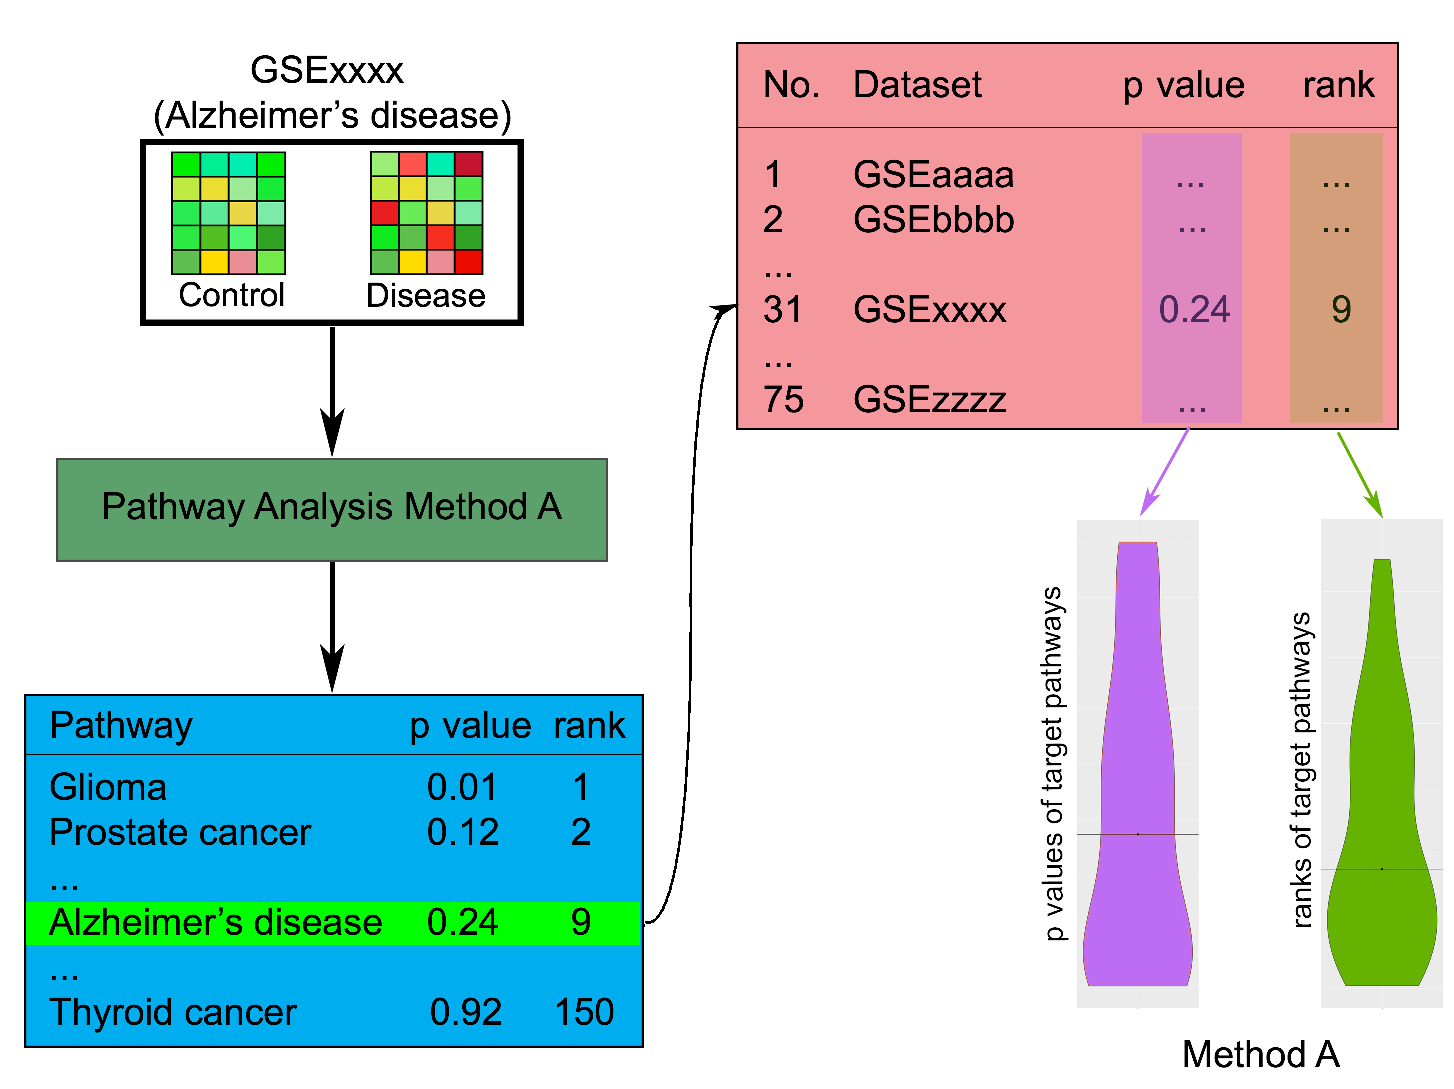
\includegraphics[width=0.8\linewidth]{Figures/Fig1}
\caption{\textbf{The process of evaluating a pathway analysis method based on their ability to identify target pathways.} Each pathway analysis method is applied on 75 data sets. Methods are evaluated based on their ability to rank the target pathways. In this example, a data set of Alzheimer's disease is examined, and thus the target pathway is ``Alzheimer's disease". Each method produces lists of ranks and p value of the target pathways, which are then used to assess its performance.}
\label{workflow}
\end{figure}

Here, we propose using 75 human data sets and 11 mouse data sets for the comparison. We also take the bias of the methods towards some conditions into consideration. To make it even fairer competition, we choose the same number of data sets per conditions. In fact, we choose 15 widely studied conditions, and 5 data sets per conditions.

Table \ref{table:HumanDatasets} provides detailed information regarding the 75 human data sets used for benchmarking methods' ability to identify target pathways. This information includes: GEO ID, disease, number of normal samples and phenotype samples,  Pubmed ID, tissue from which the samples were taken, and the platform used for the experiment.

\begin{landscape}
\setlength\LTleft{0pt}            % default: \parindent
\setlength\LTright{0pt}           % default: \fill

\centering
\small
\begin{longtable}{lp{4cm}cccp{4cm}l}
\caption{75 benchmark data sets of 15 diseases used to compare 11 methods in this paper.}\\
\hline
 \textbf{GEO ID}& \textbf{Disease/Condition} & \textbf{\#Normal} & \textbf{\#Condition} & \textbf{Pubmed ID} & \textbf{Tissue} & \textbf{Platform}  \\
 \hline
GSE781 & Renal cell carcinoma	& 5	& 12	& 14641932 &	Kidney &	HG-U133A \\
GSE14762	&Renal cell carcinoma	&12	&9	&19252501	&Kidney	&HG-U133Plus 2.0 \\
GSE6357	&Renal cell carcinoma	&12	&6	&27063186	&CD8+ T Cell	&HG-U133A\\
GSE6344	&Renal cell carcinoma	&10	&10	&17699851	&Clear cell RCC	&HG-U133A\\
GSE48352	&Renal cell carcinoma	&8	&24	&NA	&Kidney	&HG-U133Plus 2.0\\
GSE1297	&Alzheimer’s disease	&9	&7	&14769913	&Hippocampal CA1	&HG-U133A\\
GSE5281EC	&Alzheimer’s disease	&13	&10	&17077275	&Brain, Entorhinal Cortex	& HG-U133Plus 2.0\\
GSE5281HIP	&Alzheimer’s disease	&13	&10	&17077275	&Brain, hippocampus	& HG-U133Plus 2.0\\
GSE5281VCX&	Alzheimer’s disease	&12	&19	&17077275	&Brain, primary visual cortex	& HG-U133Plus 2.0\\
GSE16759	&Alzheimer’s disease&	8	&4	&20126538	&Parietal lobe	&HG-U133Plus 2.0\\
GSE3467&	Thyroid cancer	&9	&9	&16365291	&Thyroid	&HG-U133Plus 2.0\\
GSE3678	&Thyroid cancer	&7	&7	&NA	&Thyroid	&HG-U133Plus 2.0\\
GSE58545	&Thyroid cancer	&18	&27	&26625260	&Thyroid	&HG-U133A\\
GSE85457	&Thyroid cancer	&3	&4	&NA	&Thyroid	&HG-U133Plus 2.0\\
GSE58689	&Thyroid cancer	&18	&27	&26625260	&Thyroid	&HG-U133A\\
GSE3585	&Dilated cardiomyopathy	&5	&7	&17045896	&Heart, subendocardial left ventricular	&HG-U133A\\
GSE33970	&Dilated cardiomyopathy	&18	&5	&NA	&Whole blood and heart	&HG-U133Plus 2.0\\
GSE29819	&Dilated cardiomyopathy	&12	&14	&22085907	&Heart, left and right ventricular	&HG-U133Plus 2.0\\
GSE79962	&Dilated cardiomyopathy	&11	&9	&NA	&Heart	&HuGene-10st\\
GSE21610	&Dilated cardiomyopathy	&8	&42	&20460602	&Heart	&HG-U133Plus 2.0\\
GSE4107	&Colorectal cancer	&10	&12	&17317818	&Colonic mucosa	&HG-U133Plus 2.0\\
GSE8671	&Colorectal cancer	&32	&32	&18171984	&Colon	&HG-U133Plus 2.0\\
GSE9348	&Colorectal cancer	&12	&70	&20143136	&Colon	&HG-U133Plus 2.0\\
GSE23878	&Colorectal cancer	&19	&19	&21281787	&Colon	&HG-U133Plus 2.0\\
GSE4183	&Colorectal cancer	&8	&15	&18776587	&Colon	&HG-U133Plus 2.0\\
GSE6956C	&Prostate cancer	&11	&36	&18245496	&Prostate	&HG-U133A 2\\
GSE6956AA	&Prostate cancer	&7	&33	&18245496	&Prostate	&HG-U133A 2\\
GSE55945	&Prostate cancer	&7	&12	&19737960	&Prostate	&HG-U133Plus 2.0\\
GSE26910	&Prostate cancer	&6	&6	&21611158	&Prostate	&HG-U133Plus 2.0\\
GSE104749	&Prostate cancer	&4	&4	&NA	&Prostate	&HG-U133Plus 2.0\\
GSE8762	&Huntington’s disease	&10	&12	&17724341	&Lymphocyte	&HG-U133Plus 2.0\\
GSE24250	&Huntington’s disease	&6	&8	&21969577	&Venous cellular whole blood	&HG-U133A\\
GSE73655	&Huntington’s disease	&7	&13	&26756592	&Subcutaneous adipose	&HuGene-10st\\
GSE45516	&Huntington’s disease	&3	&6	&24296361	&Fibroblasts	&HG-U133Plus 2.0\\
GSE37517	&Huntington’s disease	&5	&8	&22748968	&Neural stem cell	&HuGene-10st\\
GSE9476	&Acute Myeloid Leukemia	&37	&26	&17910043	&Peripheral blood, bone marrow	&HG-U133A\\
GSE14924\_CD4	&Acute Myeloid Leukemia&	10	&10	&19710498	&CD4 T Cell	&HG-U133Plus 2.0\\
GSE14924\_CD8	&Acute Myeloid Leukemia		&11	&10	&19710498	&CD8 T Cell	&HG-U133Plus 2.0\\
GSE92778	&Acute Myeloid Leukemia	&6	&6	&29035359	&Bone marrow stroma cells	&HuGene-10st\\
GSE68172	&Acute Myeloid Leukemia	&5	&72	&NA	&LSC, HSC and leukemic bulk AML \textsuperscript{*}	&HG-U133Plus 2.0\\
GSE15471	&Pancreatic cancer	&35	&35	&19260470	&Pancreas	&HG-U133Plus 2.0\\
GSE16515	&Pancreatic cancer	&15	&15	&19732725	&Pancreas	&HG-U133Plus 2.0\\
GSE32676	&Pancreatic cancer	&7	&25	&22261810	&Pancreas		&HG-U133Plus 2.0\\
GSE28735	&Pancreatic cancer	&45	&45	&23918603	&Pancreas		&HuGene-10st\\
GSE18670	&Pancreatic cancer	&6	&18	&23157946	&Pancreas	&HG-U133Plus 2.0\\
GSE18842	&Non-small cell lung cancer	&44	&44	&20878980	&Lung	&HG-U133Plus 2.0\\
GSE19188	&Non-small cell lung cancer	&62	&91	&20421987	&Lung	&HG-U133Plus 2.0\\
GSE19804	&Non-small cell lung cancer	&60	&60&	20802022	&Lung	&HG-U133Plus 2.0\\
GSE50627	&Non-small cell lung cancer	&6	&9	&25881239	&Lung	&HuGene-10st\\
GSE6044	&Non-small cell lung cancer	&5	&31	&18992152	&Lung	&HG-Focus\\
GSE19728	&Glioma	&4	&17	&21836821	&Brain	&HG-U133Plus 2.0\\
GSE21354	&Glioma	&4	&13	&21836821	&Brain	&HG-U133Plus 2.0\\
GSE50161	&Glioma	&13	&95	&24078694	&Brain	&HG-U133Plus 2.0\\
GSE4290	&Glioma	&23	&157	 & 16616334	&Brain	&HG-U133Plus 2.0\\
GSE44971	&Glioma	&9	&49	&23660940	&Brain	&HG-U133Plus 2.0\\
GSE20153	&Parkinson’s disease	&8	&8	&20926834	&B lymphocytes from peripheral blood	&HG-U133Plus 2.0\\
GSE20291	&Parkinson’s disease	&20	&15	&15965975	&Brain	&HG-U133A\\
GSE20164	&Parkinson’s disease	&5	&6	&20926834	&Substantia nigra (midbrain)	&HG-U133A\\
GSE7621	&Parkinson’s disease	&9	&16	&17571925	&Substantia nigra (midbrain)	&HG-U133Plus 2.0\\
GSE19587	&Parkinson’s disease	&10	&12	&20837543	&Brain	&HG-U133A 2\\
GSE19420	&Type II diabetes mellitus	&12	&12	&22802091	&Skeletal muscle vastus lateralis	&HG-U133Plus 2.0\\
GSE39825	&Type II diabetes mellitus	&6	&4	&23919306	&Fibroblasts (cell culture)	&HG\_U95Av2\\
GSE26887	&Type II diabetes mellitus	&5	&7	&22427379	&Left ventricle	&HuGene-10st\\
GSE21340	&Type II diabetes mellitus	&15	&5	&23919306	&Skeletal muscle	&HG\_U95Av2\\
GSE38642	&Type II diabetes mellitus	&54	&9	&22768844	&Pancreatic islets	&HuGene-10st\\
GSE24739\_G0	&Chronic Myeloid Leukemia	&4	&8	&21436996	&Peripheral blood	&HG-U133Plus 2.0\\

GSE24739\_G1	&Chronic Myeloid Leukemia	&4	&8	&21436996	&Peripheral blood	&HG-U133Plus 2.0 \\
GSE33075	&Chronic Myeloid Leukemia	&18	&9	&22388797	&Bone marrow	&HG-U133Plus 2.0 \\
GSE24739	&Chronic Myeloid Leukemia	&8	&16	&21436996	&Peripheral blood and bone marrow	&HG-U133Plus 2.0\\
GSE1418	&Chronic Myeloid Leukemia	&6	&8	&15618956	&Bone marrow	&HG-Focus\\
GSE7305	&Endometrial cancer	&10	&10	&17640886	&Endometrium/Ovarian tissue	&HG-U133Plus 2.0\\
GSE63678	&Endometrial cancer	&5	&7	&26559525	&Endometrium	&HG-U133A\\
GSE7803	&Endometrial cancer	&10	&31	&17974957	&Cervix and squamous cervical epitheilium	&HG-U133A\\
GSE17025	&Endometrial cancer	&12	&91	&21619611	&Endometrium	&HG-U133Plus 2.0\\
GSE36389	&Endometrial cancer	&7	&13	&NA	&Endometrium	&HG-U133A\\
\hline
\multicolumn{7}{l}{\textsuperscript{*}\footnotesize{Leukemic stem cells (LSC), hematopoietic stem cells (HSCs), and AML bulk cells (CD34+CD38+, CD34-CD38+ and CD34-CD38)}}
\label{table:HumanDatasets}
\end{longtable}
\end{landscape}


%Among the widely used methods described in the previous section, we would choose eleven methods in each groups to perform on real 75 data sets to prepare their individual performances. 

\subsubsection{Ability to identify the pathways containing the cause of the phenotype on mouse data sets}
\label{KOsubsubsection}

Although the above assessment is better than the human interpretation approach or using simulated data sets, it still has some limitations: it focuses solely on one true positive, the target pathway. We do not know what other pathways are also truly impacted and therefore cannot evaluate other criteria such as the accuracy, specificity, sensitivity, and the AUC of a method. Here, we use knock-out data sets that involve using knock-out experiments (KO), where the source of the perturbation is known, i.e. the KO gene.

Table \ref{table:MouseDatasets} provides detailed information regarding the 11 benchmark KO data sets used. This information includes:  the GEO ID, symbol of KO gene, number of truly impacted pathways, number of normal samples, number of phenotype samples, Pubmed ID, tissue from which the samples were taken, and the platform used for the experiment.


We consider pathways containing the KO gene as positives and the others as negatives. After performing the pathway analysis method on this data set, a p value threshold of 0.05 is used to determine whether a pathway is significantly impacted. A true positive (TP) is a positive which is correctly identified as significant. 
Similarly, a true negative (TN) is a negative which is correctly identified as insignificant.
A false positive (FP) is a pathway that does not contain the KO gene but is reported as significant. A false negative (FN) is a pathway that contains the KO gene but is not reported as significant.
Subsequently, we calculate the accuracy, sensitivity, specificity, and AUC of methods studied using 11 KO data sets. 
We also perform a higher level comparison between the ranks and p value of the target pathways obtained by non-TB and TB methods.


\begin{landscape}
\setlength\LTleft{0pt}            % default: \parindent
\setlength\LTright{0pt}           % default: \fill
\centering
\small
\begin{longtable}{@{}llccccll@{}}
\caption{Eleven knockout benchmark data sets used to compare 10 methods in this paper.\label{table:MouseDatasets}}\\
\hline
 \textbf{GEO ID}& \textbf{KO gene} & \makecell{\textbf{\#Impacted} \\\textbf{Pathways} }& \textbf{\#Nornal} & \textbf{\#Condition}& \textbf{Pubmed ID} & \textbf{Tissue} & \textbf{Platform}  \\
 \hline
GSE22873	&Myd88	&19	&11	&8	&22075646	&Liver				&Mouse430\_2 \\
GSE6030		&Neurod1	&1	&3	&3	&17630985	&Pineal gland			&Mouse430\_2 \\
GSE29048	&Pdx1	&3	&4	&4	&22135308	&Intestinal epithelium	&Mouse430\_2\\
GSE70302	&IL1a	&20	&4	&4	&26224856	&Spinal cord			&MoGene-1\_0-st\\
GSE70302	&IL1b	&34	&4	&4	&26224856	&Spinal cord			&MoGene-1\_0-st\\
GSE58120	&IL2		&3	&6	&6	&25652593	&Myeloid dendritic cells	&MoGene-1\_0-st\\
GSE46211	&TGFBR2	&20	&12	&6	&24496627	&Anterior \& posterior palatal tissue	&Mouse430\_2\\
GSE49166     &BHLHE40	&1	&3	&3	&24699451	&CD4 T cells			&MoGene-1\_0-st\\
GSE50933	&ID3		&2	&5	&5	&24244015	&Natural killer T cells	&Mouse430\_2\\
GSE62999	&DUSP5	&1	&10	&10	&25398911	&Bone marrow			&Mouse430\_2\\
GSE57917    &ONECUR1	&2	&3	&3	&25313862	&Retinas				&Mouse430\_2\\
\hline
 \end{longtable}
\end{landscape}

\subsection{Investigation of the bias under the null}

In this benchmark, we conduct a deeper investigation into the behavior of these methods under the null hypothesis. 
Here, we create a true null hypothesis by using simulated data sets that are constructed by randomly selected healthy samples from the 75 aforementioned data sets.
We apply each method  more than 2,000 times, each time on different simulated data sets.
Each pathway then has an empirical null distribution of p values resulting from those 2,000 runs (Fig \ref{nullGeneration}).
When the null hypothesis is true, p value obtained from any sound statistical test should be uniformly distributed  between 0 and 1 \cite{barton2013correction, fodor2007towards}.
However, p value generated from many pathway analysis methods are often unimodal (biased toward 0 or 1) or bimodal (biased toward 0 and 1) (Fig. \ref{fig:Biased0} and Fig. \ref{fig:Biased1}). 

\begin{figure}
\centering
%  \captionsetup{width=.8\linewidth}

	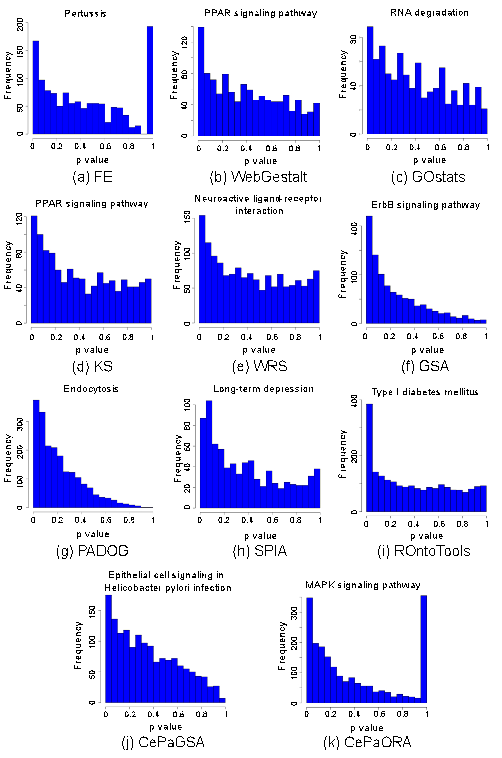
\includegraphics[width=0.8\linewidth]{Figures/Biased0}
	\caption{\textbf{Examples of pathways that have empirical null distributions of p values biased toward 0.} The procedure for generating null distributions is described in Fig. \ref{nullGeneration}. The x-axes display the p values whereas the y-axes display the frequencies. These pathways are likely to be falsely identified as significantly impacted by the corresponding method (false positive).}\label{fig:Biased0}
\end{figure}

\begin{figure}
\centering
%  \captionsetup{width=.8\linewidth}

	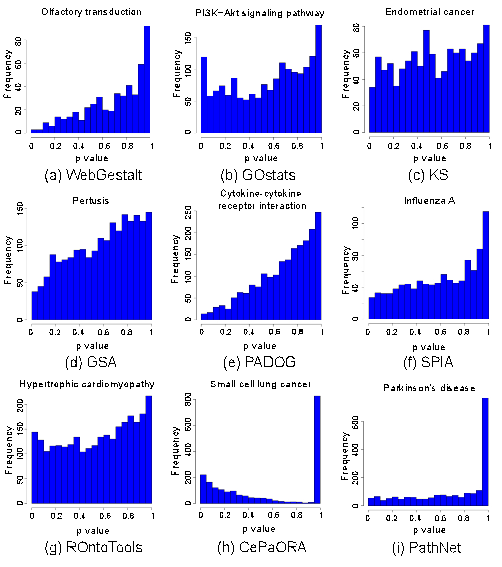
\includegraphics[width=1\linewidth]{Figures/Biased1}
	\caption{\textbf{Examples of pathways that have empirical null distributions of p values biased toward 1.} In these sub-figures, x-axes represent the p value, while y-axes represent their frequencies. These pathways are often incorrectly excluded in the list of significant pathways  by the corresponding method even when they are indeed impacted (false negative).}\label{fig:Biased1}
\end{figure}


More specifically, a null distribution of p value of a pathway generated by a method skewed to the right (biased toward 0) shows that this method has a tendency to yield low p value and therefore report the pathway as significantly impacted even when it is not (false positive). By contrast, a null distribution of p value of a pathway skewed to the left (biased toward 1) indicates that the given method tends to produce consistently higher p value thus possibly report this pathway as insignificant when it is indeed impacted (false negative).
The results of this null-hypothesis analysis may explain why some methods work well for certain diseases while they perform poorly for others. If a method is biased to report more often a given cancer pathway as significant, that method may be perceived to perform better in experiments involving that particular type of cancer. 

\begin{figure}
\centering
	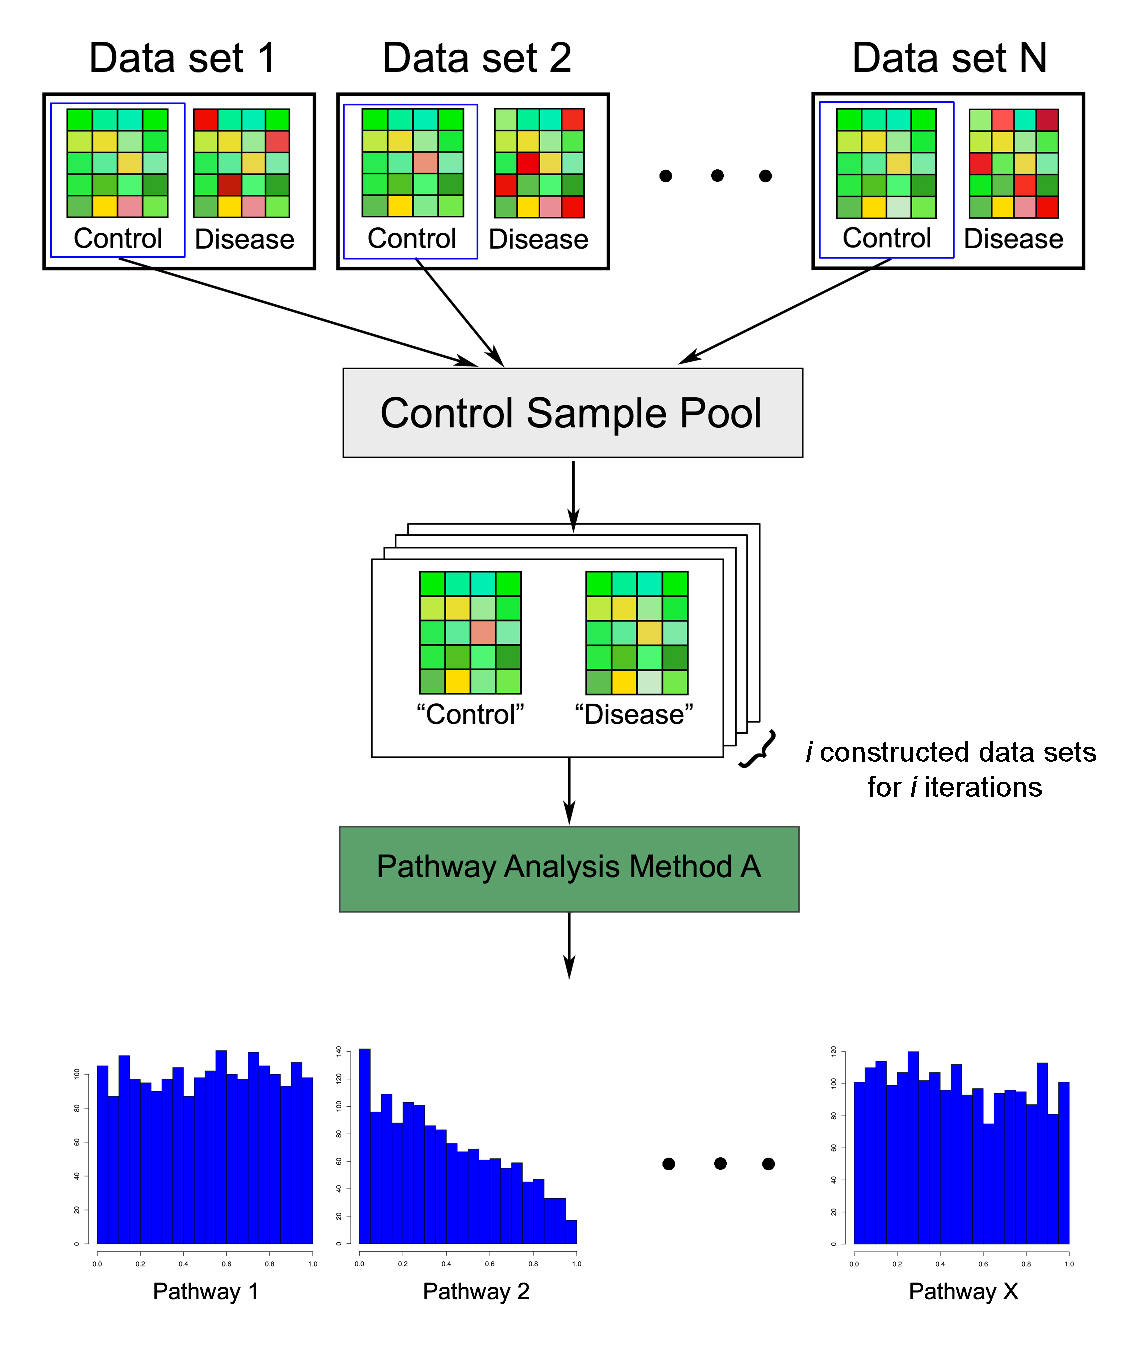
\includegraphics[width=0.8\linewidth]{Figures/Fig4}
  \caption{\textbf{The process of creating the null distributions of p value for all pathways by a given pathway analysis method.} Control samples from data sets are  gathered to construct a control sample pool. To create the null distribution of p value of all pathways under the null for each method, more than 2,000 iterations were performed. The data sets used in these iterations are generated by randomly selecting samples from the control sample pool.}
  \label{nullGeneration}
\end{figure}

We would also report the total number of biased pathways  (either toward 0 or 1) produced by these methods.
%The number of biased pathways is at least 66 for all the methods compared in this work, except GSEA which has no biased pathway was found. 
%While investigating more, we found that the aggregate p value of all the pathways generated by GSEA is uniformly distributed under the null (Additional file 1: Fig. \ref{fig:GSEAagg}).
%A similar conclusion about GSEA was also reached by Nguyen \textit{et al.}~\cite{nguyen2017DANUBE}.

%The number of pathways biased toward 0 produced by 13 methods are shown in Figure \ref{fig:NumberOfBias}b.
%The figure shows that performing pathway analysis using FE test produces the highest number (137 out of 150 pathways) of false positives, this is followed by WRS test (114 out of 150 pathways) and CePaGSA (112 out of 186 pathways). On the other hand, GSEA and PathNet produce no false positive pathways.
%
%Similarly, the numbers of pathways biased toward 1 produced by different methods are shown in Figure \ref{fig:NumberOfBias}c.
%PathNet produces the highest number (129 out of 130 pathways) of false negative pathways.
%No false negative pathways are identified while performing pathway analysis using GSEA, CePaGSA, WRS test and FE test.

%\begin{figure}[!h]
%	\includegraphics[width=0.7\linewidth]{picturesForGB/NrBiasedPathway}
%        \caption{\csentence{The number of biased pathways calculated based on Pearson's moment coefficient.}  Under the true null hypothesis, an ideal method would produce a uniform distribution of p value from 0 to 1 for every pathway. Here, thresholds of Pearson's moment coefficient of $0.1$ and $-0.1$ are used to determine if the empirical distribution p values is biased toward 0 or 1, respectively.
%        Panel (a) shows the total number of biased  pathways (toward either 0 or 1) produced by each method.
%Each method, except GSEA, has at least 66 biased pathways.
%Panel (b) shows the number of pathways biased toward 0 (false positives) produced by different methods.
%FE  produces the highest number (137 out of 150 pathways) of false positives, followed by WRS  (114 out of 150) and CePaGSA (112 out of 186).
%Panel (c) shows the number of pathways biased toward 1 (false negatives) produced by different methods.
%PathNet produces the highest number (129 out of 130) of false negative pathways. The methods in red are TB methods. The methods in blue are non-TB methods}\label{fig:NumberOfBias}
%\end{figure}


%\begin{figure}[h]
%	\includegraphics[width=0.8\linewidth]{picturesForGB/NrMethodsBiased}
%
%        \caption{\csentence{The number of methods biased for each pathway.} The y-axis shows the KEGG pathways, while the x-axis indicates the number of methods biased toward 0 and  1, respectively. Each horizontal line represents a pathway. The lengths of the blue and red lines show the number of methods in this study biased toward 0 and 1, respectively. Pathways are sorted by the number of methods biased. There is no pathway that is unbiased for all methods. The top 10 least and top 10 most biased pathways are shown by name.}\label{fig:PathwaysDist}
%\end{figure}




\clearpage

\section{Predicting upstream regulator approach for drug repurposing and causal analysis}



\label{chap:PURE}

%\subsection{Introduction}


%In this article, we describe a novel tool for Predicting Upstream REgulators (PURE) that can perform a causal analysis and infer the cause of a set of measured gene expression changes. 
In this chapter, we describe a novel causal analysis tool for predicting upstream regulators that can infer the cause of a set of measured gene expression changes. 
Given a set of differentially expressed genes between samples with studied phenotype and control samples, we would analyzes more  than 5,000 CDTs and their 330,659 known associations with human genome, 187,759 associations with mouse genome, and 161,323 associations with the rat genome as described in the Comparative Toxicogenomics Database~\cite{mattingly2006comparative}. 
 
% \hfill
 
In the following subsections, we present the hypotheses tested in the study and the approach to calculate the significance score for each hypothesis.
%We propose  assessment criteria of the performance of PURE and compare it with four classical methods, namely Over Representation Analysis using hypergeometric test~\cite{DraghiciOE2:2003}, Kolmogorov-Smirnov (KS)\cite{massey1951kolmogorov}, Wilcoxon\cite{wilcoxon1945individual}, FGSEA~\cite{korotkevich2021fast}, and a commercial tool, namely Ingenuity Pathway Analysis~\cite{kramer2013causal}. 
%The result shows that our method outperforms existing methods in term of both the ability of identifying the causal CDT, as well as in terms of the number of false positives yielded by each method.

%\subsection{Methods}

\subsection{Knowledge base}
First, we would preprocess the network of drug-gene interactions from the Comparative Toxicogenomics Database~\cite{mattingly2006comparative} that provides manually curated information about associations between more than 5,000 CDTs and tens of thousands of genes from many species including human, mouse, rat, etc. These data include the chemical family, the CDT-gene, and CDT-disease relationships.
There are various types of relationships between a CDT and targeted or affected genes, such as increase/decrease expression, increase/decrease abundance, or increase/decrease methylation.
In this analysis, since our goal is to analyze gene expression measurements, we would focus on  those effects leading to an expression increase or decrease. Henceforth, these will be referred to as ``activation'' and ``inhibition'' effects.



\subsection{Two hypotheses}

For each CDT in the database, we would consider two hypotheses:

\begin{itemize}
\item Hypothesis 1 (H1): the level of the CDT is higher in the phenotype compared to the control.%; and hence, enhances expressions of the downstream genes via the direct interaction edges.
\item Hypothesis 2 (H2): the level of the CDT  is lower  in the phenotype compared to the control (or completely absent).%; and hence, the downstream genes are not regulated properly.
\end{itemize}

\subsection{Statistical significance}


Let $G_{DE}$ be the set of differentially expressed genes available in the gene expression profile; $C_{KB}$ be the set of all CDTs in the knowledge base (KB); $G_{KB}$ be the set of genes in the KB, and $E_{KB}$ be the set of edges that represents the associations between CDTs and genes in the KB. 
%where $A \in C_{CTD}$ is a chemical, $x \in G_{CTD}$ reflects a gene, and an edge $e_{A,x} \in E_{CTD}$ represents a relationship between the drug $A$ and gene $x$.

\begin{figure*}
\centering
  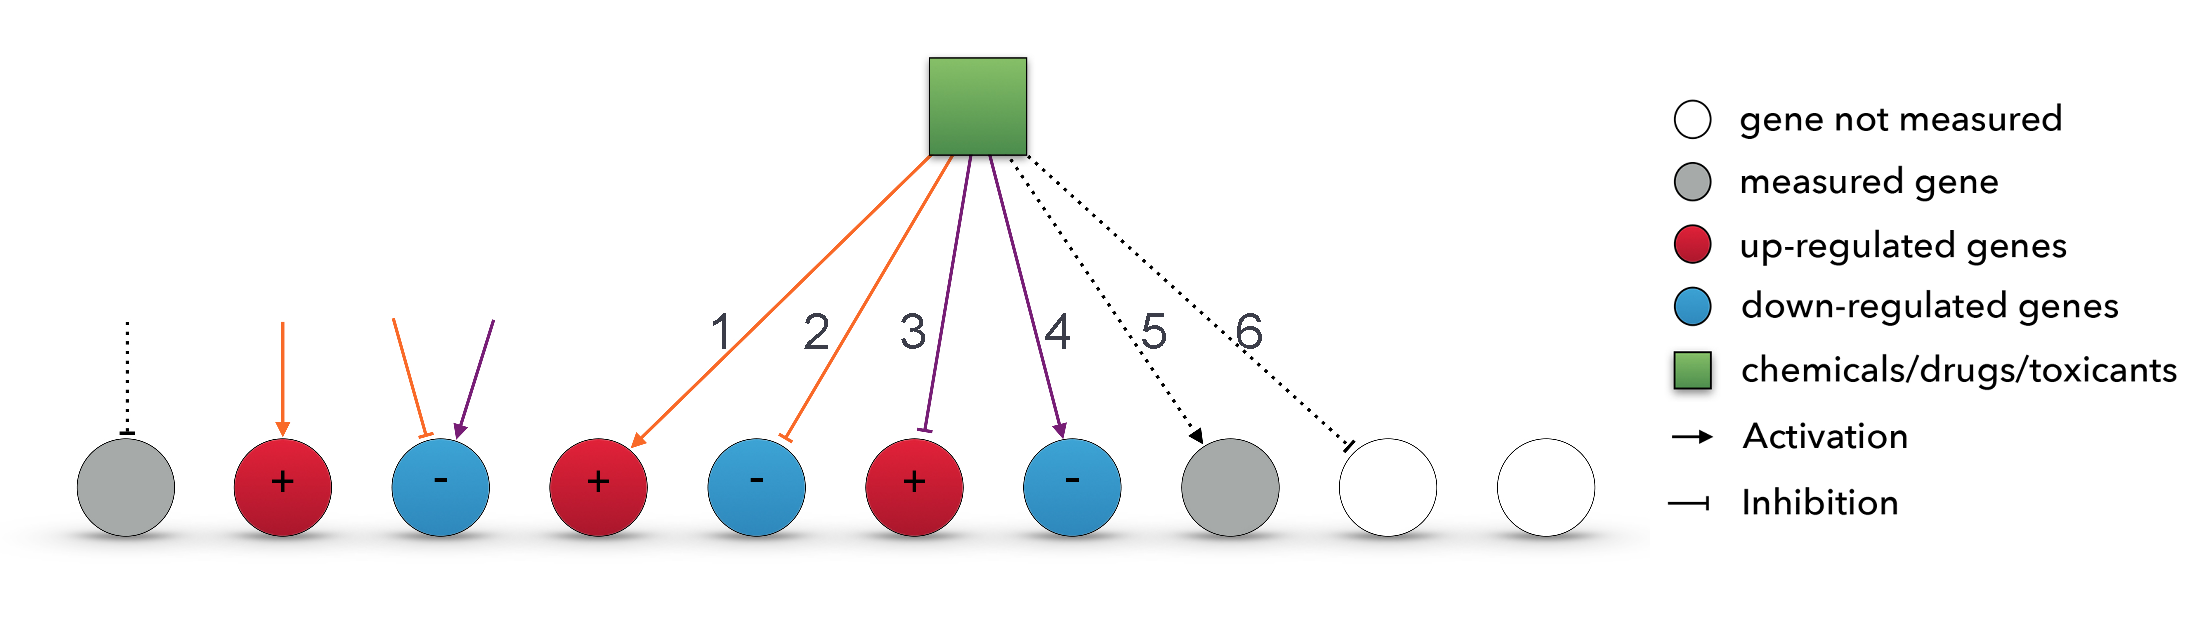
\includegraphics[width=1\linewidth]{Figures/SecondEvidence.pdf}
  \caption{Illustration of different types of genes available in the Comparative Toxicogenomics Database and gene expression profile, and their relationships with the chemical. The significance of a chemical/drug/toxicant (green box) in each hypothesis is assessed using a statistical test based on the number of up- or down-regulated DE genes and their associations with the drug. The orange edges (e.g. 1 and 2) are the ones that support the hypothesis that level of studied chemical/drug/toxicant is higher in the phenotype compared to the control while the purple ones (e.g. 3 and 4) are supporting the hypothesis that its level is lower compared to the control.}
  \label{fig:SignificantDrug}
\end{figure*}

We define G as  the set of genes included in both $G_{DE}$ and $G_{KB}$, i.e.  $G_{DE} \cap G_{KB}$. Subsequently, $C \subseteq C_{KB}$  and $E \subseteq E_{KB}$ represent the set of all CDTs and their corresponding associations with those genes in $G$ available in the knowledge base. These sets are formally defined as follows:

\begin{equation}C = \{c \in C_{KB} \mid \exists g \in G \land \exists e_{c,g} \in E_{KB} \}\end{equation}

and 

\begin{equation} E = \{ e_{c,g} \mid \exists c \in C \land  \exists g \in G \ \land  e_{c,g} \in E_{KB} \} \end{equation}

%Let $G^{+}\subseteq G$ and $G^{-}\subseteq G$ be the list of up- and down-regulated DE genes, respectively. 

where $e_{c,g}$ denotes an edge from an upstream CDTs $c$ to targeted gene $g$ representing their relationship described in the Comparative Toxicogenomics Database. The sign of the edge, $s(e_{c,g})$, reflects the type of the association, namely positive ($+$) for an activation and negative ($-$) for an inhibition edge. Also, we denote $s(g)$ the sign of the DE gene $g$ which is positive if $g$ is up-regulated, and negative, otherwise. 

Each edge $e \in E$ is labeled whether it is supporting either of the testing hypotheses (Fig.~\ref{fig:SignificantDrug}). 
For example, if an edge is activation and its targeted DE gene is indeed up-regulated, the edge supports the hypothesis 1. 
%Similarly, an inhibition edge connected with a down-regulated DE gene is also backing this hypothesis. 
In essence, an edge is considered to be supporting the hypothesis 1 when its sign, $s(e_{c,x})$, is aligned with the sign of its targeted DE gene, namely $s(e_{c,g}) = s(g)$. 
Such edges are colored orange in Fig.~\ref{fig:SignificantDrug}. 
Edges whose signs are opposite with the expression direction of their targeted DE genes are considered as a supporting evidence for the hypothesis 2, and are colored purple in  Fig.~\ref{fig:SignificantDrug}. 
Notice that $E^{H1}$ and $E^{H2}$ are the two mutually exclusive sets of edges that support the first and second hypothesis, respectively, because an edge $e \in E$ must support either the hypothesis 1 or hypothesis 2, but not both. Formally, $E^{H1} \cap E^{H2} = \emptyset$ and  $E^{H1} \cup E^{H2} = E$. 

For each chemical $c \in C$, a statistical score, i.e. p value, for each aforementioned hypothesis is then computed using the one-sided Fisher's exact test. Without losing generality, let us discuss the hypothesis 1. First, a confusion matrix is constructed as in Table \ref{ConfusionMatrix}, where $l$, $k$, $m$, and $n$ are the number of edges related to $c$ that support the hypothesis, the number of edges related to $c$ that do not support the hypothesis, the number of edges not related to $c$ that support the hypothesis, and the number of edges not related to $c$ that do not support the hypothesis, respectively. 
The probability of this observed contingency under the null hypothesis is defined as follows:
\begin{equation}
p = \frac{ {l+k \choose l}{m+n \choose m}}{{\|E\| \choose l + m}}
\end{equation}
where $\|E\| = (l+k+m+n)$ is the number all edges in $E$. 

The p value of the one-sided Fisher's exact test is the sum of the probabilities of all contingency tables that have the number of edges supporting the H1 more than $l$ where the number of edges related to the compound C and the number of edges supporting the H1 are unchanged.

Notice that because an edge supporting H1 is against H2 and vice versa, the contingency matrix for H2 can be obtained by swapping the columns of the observed contingency matrix of H1. Hence, the p value for the H2 can also be derived from these four numbers.


Finally, we use the false discovery rate (FDR) to correct the p values for multiple comparisons~\cite{Benjamini:1997}.

\begin{table}
\caption{For each chemical/drug/toxicant $c$, a contingency table is constructed. Here, \emph{l}, \emph{k}, \emph{m}, and \emph{n} are the number of edges coming from $c$ that support the hypothesis 1 (H1), the number of edges coming from $c$ that do not support the H1, the number of edges not coming from $c$ that support the H1, and the number of edges not coming from $c$ that do not support the H1, respectively. Note that the edges that support H1 are against the hypothesis 2 (H2), and vice versa. Hence, a similar contingency table for H2 can be constructed using these four numbers.}
\begin{center}
\begin{tabular}{c|cc}
&  Supporting H1& Against H1\\
\hline
Related to $c$& \emph{l} & \emph{k} \\
 Not related to $c$&\emph{m}& \emph{n}  \\
%\hline 
%Total & $\|E1\|$ & $\|E2\|$ & $\|E\|$
\end{tabular}
\end{center}
\label{ConfusionMatrix}
\end{table}%






%\subsection{Conclusion}
%
%The most important contribution of PURE is that it can infer the CDT responsible for the gene expression changes, which in turn causes the observed phenotype. This crucial ability is expected to be useful for the correct identification of the presence of chemicals, drugs or toxicants in new and unknown phenotypes.  Moreover, PURE can identify the CDT that can revert disease-induced gene expression changes. This capability is expected to be useful in any drug repurposing application. In fact, this approach coupled with a pathway analysis, was able to repurpose methylprednisolone to treat severe symptoms related to hyper-inflammation of COVID-19 patients, very early in the pandemic, at a time when the WHO's recommendation was against the use of steroids~\cite{DraghiciCOVID:2021}.
% 
%The proposed approach was validated using 16 gene expression data sets from 3 different species where the true CDTs that caused the phenotypes were known. PURE correctly identified the CDT used in 11 out of 16 data sets (7 of which the true CDTs were ranked at the top). We also compared PURE to 5 other methods including a commercial tool, IPA. PURE outperformed all other methods in terms of the rank of the true CDT and the number of false positives in the list of significant CDTs.
\clearpage



\subsection{Proposed validation}

In this chapter, we discuss our approach to validate the proposed method and compare it with existing methods with some benchmarking data sets. The competitive methods are ORA, Kolmogorov-Smirnov test, Wilcoxon, FGSEA, and IPA. We describe 16 data sets from three species, namely human, mouse, and rat, with 8 different CDTs used for methods comparison. %Out of these 16 data sets, 14 data sets are used for testing the hypothesis 1, and the other two are used for validating the hypothesis 2.

\subsubsection{Benchmarking methods}
%\subsubsection{}

The ORA family of methods, as well as other tests, such as KS, Wilcoxon, and FGSEA, are widely used in gene set analysis to determine whether  a particular gene set - such as the genes associated to a given GO term or pathway - is significantly affected in the given phenotype. In principle, the same approach could be used to decide whether a given CDT could be related to the phenotype by considering the set of genes known to be affected by the given CDT. 

\textbf{ORA} uses a statistical test, such as hypergeometric, chi-square, or binomial distribution, to evaluate if the number of DE genes is over- or under-represented in the set of targeted genes of a CDT. In this study, we would use hypergeometric test to compute p value, namely the probability of getting the $x$ or more observed DE genes in $M$ CDT's downstream genes from a pool of $N$ background genes with $n$ DE genes. Mathematically, this probability is defined as:

\begin{equation*}
P(X \geq x) = 1-P(X \leq x -1)= 1- \sum_{i=0}^{x-1} \frac{\binom{M}{i}\binom{N-M}{n-i}}{\binom{N}{n}} 
\end{equation*}

ORA does not take into consideration if the DE gene is up-regulated or down-regulated, nor the type of associations between the CDT and the targeted DE gene.

The Kolmogorov-Smirnov test (\textbf{KS}) determines whether there is a significantly difference between two empirical distributions of the scores (the direction of the fold changes) of the DE genes targeted by the CDT (\texttt{DEhit}) and those of the DE genes not targeted by the CDT (\texttt{DEmiss}). First, all genes will be ranked in order of their log fold changes. Then, we calculate the cumulative distribution function (CDF) of the ranked gene list for background genes and for the genes affected by the CDT. Finally, the KS test is used to compare the two CDFs and calculates a p value that measures the significance of the enrichment. Although KS takes the sign of the DE genes into consideration (the fold changes of gene expression), it ignores the type of associations between CDTs and DE genes.

\textbf{Wilcoxon} is a rank-based non-parametric test for comparing the ranks of DE genes affected by the CDT (\texttt{DEhit}), and other DE genes (\texttt{DEmiss}). First, it ranks all genes in both lists based on their fold changes. Subsequently, it computes the a test statistic $W$, which is the sum of the ranks for all \texttt{DEhit}. This test statistic $W$ is compared to the distribution of $W$ under the null hypothesis. The null hypothesis is rejected if $W$ is extreme and falls outside 95\% of the distribution. In R, the Wilcoxon is available via the function \texttt{wilcox.test}.  Similar to ORA, the  associations of the affected DE genes with the CDT are completely ignored.

\textbf{FGSEA} is an improvement of the Gene Set Enrichment Analysis (GSEA) approach. FGSEA accelerates the calculation of the GSEA p value by estimating it with a high accuracy (the estimation error is less than $10^{-100}$ when compared with actual GSEA p value). GSEA, in turn, is one of the most popular approaches in gene set analysis\cite{Subramanian:2005}. It consists of three important steps: computing the enrichment score for each gene set, estimating the statistical significance of the enrichment score, and adjusting for multiple hypothesis testing. We used the function \texttt{fgsea} in the ``fgsea'' package with the parameters \texttt{nperm = 10\textsuperscript{4}} and \texttt{minSize = 15}.

\textbf{IPA} is a commercial web-based platform that offers several applications including a causal analysis tool\cite{kramer2013causal}. Given a list of DE genes, IPA's causal analysis outputs a list of upstream regulators including chemicals/drugs, as well as genes, proteins families, complexes, microRNA, and biological processes.
Notice that including all these types of regulators in the report would worsen the IPA's result when benchmarking with other methods since it might increase the rank of the true CDT. Moreover, since there is only one true causal CDT in each experiment and all other elements are considered as false positives, having them in the result would increase the number of false positives. 
For these reasons, beside the default IPA result, we added to the method benchmarking the so-called IPA-CDT  that only retains the CDTs in the IPA report and excludes all non-chemical elements.

According to Kr\"{a}mer \textit{et al.}, IPA derives two scores for each regulator \textit{r}, namely the overlap p-value and the activation z-score, as follows.

\emph{The overlap p-value} reflects the enrichment of the list of \textit{r}-regulated genes in the set of all DE genes without taking the regulation direction into consideration. Formally, it is based on the one-sided Fisher's exact test and is calculated as follows:

\begin{equation*}
p(r)=\sum_{k = 0}^{min(c,d)} \frac{(a+b)!(c+d)!(a+c)!(b+d)!}{(a+k)!(b-k)!(c-k)!(d+k)!n!}
\end{equation*}

where $n$ is the number of all background genes, i.e. all the genes in the data set that have at least one association with any upstream regulator, $a$ is the number of DE genes regulated by $r$, $b$ is the number of DE genes that are not regulated by $r$, $c$ is the number of $r$-regulated genes but not differentially expressed, and $d=n-a-b-c$.

\emph{The activation z-score} uses the information about the direction of gene regulation to predict the regulators. Let $\tilde{O}$ be the set of $r$-regulated DE genes, the activation z-score of the corresponding regulator $r$ is defined as:


\begin{equation*}
z(r) =  \frac{\sum\limits_{v \in \tilde{O}}w_{R}(r,v) s_{R}(r,v) s_{D}(v)}{\left(\sum\limits_{v \in \tilde{O}}[w_{R}(r,v)]^2\right)^{1/2}}
\end{equation*}

where $w_{R}(r,v)$ represents the weight associated with the regulation of $r$ and the downstream DE gene $v$, $s_{R}(r,v)$ is the sign of the regulation, i.e. $s_{R}(r,v)=1$ for activation and $s_{R}(r,v)=-1$ for inhibition, and $s_{D}(v)$ represents the direction of DE gene's expression, i.e. $s_{D}(v)=1$ for up-regulation and $s_{D}(v)=-1$ for down-regulation, respectively. The activation z-score is proven to be approximately normally distributed under the null model, e.g. random signs $s_{R}(r,v)$ and $s_{D}(v)$. On one hand, a high positive z-score, e.g. $z(r) > 2$, indicates that the match between the signs of downstream DE genes ($s_{D}(v)$) and the corresponding edges ($s_{R}(r,v)$) is significant, which in turn suggests that $r$ is the activated regulator. On the other hand, a low negative z-score, e.g. $z(r) <  -2$, is an indicator that the sign of the downstream DE genes are mostly opposite with the corresponding regulations. In this case, $r$ is predicted as an inhibitor~\cite{kramer2013causal}.




\subsubsection{Validation data sets}

We downloaded 16 benchmark data sets from Gene Expression Omnibus database (GEO: \url{https://www.ncbi.nlm.nih.gov/geo/}). 
%These data sets are experiments in which gene expressions of control samples are compared with samples exposed to a studied CDT. 
These experiments varied from human, mouse, to rat with 8 different CDTs (See Table~\ref{Datasets}).

The DE genes are selected using a threshold of $|log(FC)| > 0.6$ and $p\ value < 0.05$.

Out of these 16 data sets, the first 14 data sets are used for testing the hypothesis 1, and the other two are used for validating the hypothesis 2.


\begin{table}
\caption{The detailed information of 16 benchmarking data sets used in this manuscript. All data sets are downloaded from Gene Expression Omnibus (GEO) database.}
\label{Datasets} 
\begin{center}
\scriptsize
\begin{tabular}{ c|cccc } 

 \hline \hline
Experiment ID & GEO ID& Organism& True CDT  &Hypothesis\\ 
\hline
1  & GSE26487~\cite{stojadinovic2007novel}& Human & Dexamethasone & H1 \\ 
2  & GSE49804~\cite{peffer2014caveolin}& Mouse & Dexamethasone & H1\\ 
3  & GSE86837~\cite{stenz2017testicular}& Mouse & Diethylhexyl Phthalate &H1\\ 
4  & GSE58434\_H~\cite{himes2015vitamin}$^{(1)}$& Human & Calcitriol (Vitamin D) &H1\\ 
5  & GSE58434\_Ast~\cite{himes2015vitamin}$^{(2)}$& Human & Calcitriol (Vitamin D)  &H1\\ 
6  & GSE11352\_12h~\cite{lin2007whole} & Human & Estradiol  &H1\\ 
7  & GSE11352\_24h~\cite{lin2007whole}& Human & Estradiol &H1 \\ 
8  & GSE11352\_48h~\cite{lin2007whole} & Human & Estradiol &H1\\ 
9  & GSE74000~\cite{rodrigues2016gene} & Human & Acetaminophen &H1\\ 
10 & GSE12446~\cite{Hanifi-Moghaddam:2007} & Human & Estradiol &H1\\
11 & GSE67266\_WT$^{(3)}$	& Mouse	& Etoposide &H1\\
12 & GSE67266\_KO$^{(4)}$ &	Mouse &	Etoposide &H1 \\
13 & GSE51213	& Mouse	& Dexamethasone&H1\\
14 & GSE58875~\cite{tallino2015nutrigenomics}	& Rat & Copper deficiency &H1\\
15 & GSE147507\_NHBE~\cite{Blanco-Melo:2020}$^{(5)}$ & Human & Methylprednisolone&H2\\
16 & GSE147507\_A549~\cite{Blanco-Melo:2020}$^{(6)}$ & Human & Methylprednisolone&H2\\
 \hline\hline
 \multicolumn{5}{l}{\tiny $^{(1)}$ Contrast: Healthy patient treated with vitamin D vs healthy patient untreated}\\
 \multicolumn{5}{l}{\tiny $^{(2)}$ Contrast: Asthma patient treated with vitamin D vs asthma patient untreated}\\
 \multicolumn{5}{l}{\tiny $^{(3)}$ Contrast: Wild Type (WT) mice treated with etoposide vs mock treated after 6 hours}\\
 \multicolumn{5}{l}{\tiny $^{(4)}$ Contrast: MK2/3 knockout (KO) mice treated with etoposide vs mock treated after 6 hours}\\
 \multicolumn{5}{l}{\tiny $^{(5)}$ Contrast: Primary normal human bronchial epithelial cells (NHBE) infected with COVID-19 vs control}\\
 \multicolumn{5}{l}{\tiny $^{(6)}$ Contrast: A549 lung cell line infected with COVID-19 versus control}\\
\end{tabular}
\end{center}
\end{table}


\subsubsection{Assessment criteria}

%\subsubsection{Assessment}

We would evaluate and compare the performance of our proposed method with the other five approaches, namely Over Representation Analysis (ORA) using hypergeometric test, Kolmogorov-Smirnov test (KS)\cite{massey1951kolmogorov}, Wilcoxon\cite{wilcoxon1945individual}, FGSEA~\cite{korotkevich2021fast}, and the causal analysis used in Ingenuity Pathway Analysis (IPA)~\cite{kramer2013causal}.



\textbf{Assessment of hypothesis 1}

We would evaluate these methods using 14 benchmark data sets from three different species, namely human, mouse, and rat (See Table \ref{Datasets}, experiment ID from 1 - 14). 
In these data sets, gene expressions were measured after the ingestion of a given CDT.
Hence, the cause of all the changes observed  throughout the system is known. Furthermore, this particular situation corresponds to  H1, where the level of the CDT is higher than normal.
We consider the administered CDT as the ``true CDT'' for each of these data sets.

The result of each method is a ranked list of CDTs based on the particular statistic used by each method, i.e. FDR-adjusted p values for our proposed method, ORA, KS, Wilcoxon, and FGSEA, and  z-score  for IPA and IPA-CDT. 
If several CDTs are ranked with the same statistic, we use an average. For instance, if  the top 4 elements have the same p value, they would be all ranked as 2.5 instead of 1, 2, 3, and 4, respectively because 2.5 is the average of the set $\{1, 2, 3, 4\}$.
An ideal method would be able to identify the true CDT by ranking it on top with a significant p value $\leq 0.05$ or  z-score $\geq 2$ (or z-score $\leq -2$ in case of IPA testing the H2).

%There are 14 data sets corresponding to the H1 where the causal CDTs are known (Table~\ref{Datasets}). We report and compare the ranks of the true CDTs in these 14 data sets (see Table~\ref{Ranks} and Fig.~\ref{fig:resultFigure}a).
%PURE (average = 2.8) is better than all of the methods in this study, followed by IPA-CDT (average = 17.7), ORA (average = 20.1), and KS (average = 24), GSEA (average = 32.9), IPA (average = 79.9), and Wilcoxon (average = 104.4) (Table \ref{Ranks}). PURE can successfully identify the true CDTs in these 14 benchmarking data sets and rank them at the top 7 times. It performs better than all of the methods in 9 data sets. IPA-CDT performs best in 6 data sets (3 of which are tied with PURE) and is able to rank the true CDTs at the top 5 times. However, it cannot identify the true CDTs in three data sets, in two of which the true CDTs are not present in the result list (data set 8 and data set 14). Similar to IPA-CDT, IPA can correctly rank the true CDTs at the top in 5 data sets.  FGSEA performs best in 2 data sets. ORA performs best in one data sets (tied with PURE), while KS and Wilcoxon are not able to perform best in any of the experiment.


Notice that an evaluation based solely on the method's ability to identify the true CDT using the p value does not show the whole story and sometimes misleads.
For example, a method that derives low p values for all CDTs can always identify the true CDT, but is still considered a bad one because it includes a lot of false positives in the result.
Therefore, we would also take the number of false positives in the result into consideration, i.e. the number of CDTs that are not true CDT but reported as significant. % (Fig. \ref{fig:resultFigure}b).
Although chemicals and drugs could have similar effects or could be in the same family, we only consider the true CDT as the one and only true positive and all other CDTs as true negatives.
We expect a good method would derive a low number of CDTs in the result, ideally only one, the true CDT.
%Our method generally reports the lower numbers of reported chemicals (average = 19.4) than any other methods compared, followed by FGSEA (average = 37.4) and IPA-CDT (average = 37.6).
%Although FGSEA is comparable to IPA-CDT, it cannot identify the true CDTs in 6 out of 14 experiments while IPA  cannot identify only 3 out of 15.
%Wilcoxon and IPA report on average more than 100 CDTs while ORA and KS report on average more than 200 CDTs per experiment (Table \ref{NrSig}).


%e.g in the experiment 9 performed by IPA, we assigned 31 to the true CDT's rank because IPA reported a list of 30 significant CDTs but the true CDTs is not included (Table ~\ref{NrSig}). 
%The p value for the number of CDTs reported comparison between PURE and IPA-CDT, ORA, KS,  FGSEA, IPA, and Wilcoxon are 0.04, 4E-4, 9E-6, 0.4, 4E-5, and 2E-6, respectively. 
%Since all  p values are less than the standard threshold of 0.05 (except for FGSEA while comparing the number of CDTs reported), PURE's performance can be considered significantly better than all of the methods included in the study, in terms of both the rank of the true CDTs, as well as the number of significant CDTs reported.

\textbf{Assessment of hypothesis 2}

The assessment of these methods on testing H2 is more challenging since the data sets in which the ground truth is known are scant, i.e. an CDT is truly lacking in the system. Another important application for testing the H2 is drug repurposing. A CDT could potentially reverse the  gene expression changes caused by the disease and therefore be a candidate for drug repurposing. 
%Similar approach using the data set GSE147507, in which the expression of NHBE and A549 cells infected with COVID-19 were compared with their corresponding control, proposed Methylprednisolone to improve the outcome in server COVID-19 cases~\cite{DraghiciCOVID:2021}. This finding was aligned with several clinical trials from different research groups~\cite{DraghiciCOVID:2021, corral2021methylprednisolone,salton2020prolonged, meduri2020pharmacological}. 
%At the time we applied PURE to the COVID-19 data, the recommendation of several organizations, including the World Health Organization (WHO), CDC, and Surviving Sepsis Campaign, was against the use of any systemic corticosteroids in the severe cases of COVID-19~\cite{wilson2020covid}. 
%Surprisingly, our results showed that Methylprednisolone, a corticosteroid, would be effective in helping the patients with severe disease~\cite{DraghiciCOVID:2021}. 


During COVID-19 pandemic in 2020,  researchers around the world were focusing to find a drug that treats the COVID-19. For the short period of time, the popular and feasible approach at the time was drug repurposing. Clinical trials have shown that  steroids are effective \cite{meduri2020pharmacological, corral2021methylprednisolone,salton2020prolonged, meduri2020pharmacological, cochrane1996systemic, prescott2020corticosteroids}, and the World Health Organization (WHO) has reversed their previous recommendation against the use of any systemic corticosteroids in the severe cases of COVID-19~\cite{wilson2020covid}. At this time, the standard of care in severe cases of COVID-19 is the corticosteroid treatment. 
Hence, in this study, we would use the data set GSE147507 in which the expression of NHBE and A549 cells infected with COVID-19 were compared with their corresponding control, and consider Methylprednisolone as the ``target'' CDT in the experiments 15 and 16 for different contrasts. %(Table~\ref{H2Result}).

Similarly to testing the H1, we would validate whether a method can identify the target CDT and has as few false positives as possible.
%PURE can identify the true CDTs in all of the experiments.
%Also notice that in data set 13, IPA could determine the target chemical, dexamethasone, as significant and rank it 13, there are 173 other false positive chemicals in the result.
%

%
%\begin{table}
%\caption{\label{Ranks} Benchmarking the methods in term of the ranks of the true CDTs. The experiment IDs (Exp. ID) are corresponding to the ones in Table \ref{Datasets}. The lower the rank of the true CDTs, the better.  The green highlighted cell is the best one in each experiment. PURE performs best in 9 out of 14 experiments, followed by IPA which performs best in 6 experiments (3 co-best with PURE). In two of the data sets analyzed IPA was not able to identify the correct CDT at all  (highlighted in red).}
%\begin{center}
%\scriptsize
%\begin{tabular}{ ccc|ccccccc } 
%
% \hline \hline
%
%\multirow{2}{*}{Exp. ID}& \multirow{2}{*}{GEO ID}& \multirow{2}{*}{Organism} & \multicolumn{7}{c}{\textbf{Rank of true CDTs}} \\
%&  && PURE  & ORA & KS  & Wilcoxon & FGSEA & IPA& IPA-CDT\\
%\hline
%1	& GSE26487& Human &	\cellcolor{green}1	&	1.5	&	43	&	45	&	25.5	& \cellcolor{green}1&	\cellcolor{green}1\\ 
%
%2	& GSE49804& Mouse	&	2	&	2	&	33	&	11	&	16.5	&	\cellcolor{green}1 & \cellcolor{green}1\\ 
%
%3	& GSE86837& Mouse	&	\cellcolor{green}1	&	\cellcolor{green}1	&	3	&	2.5	&	47	&	816& 153\\ 
%
%4	& GSE58434\_H& Human &	\cellcolor{green}1	&	16	&	13.5	&	65	&	159	&	25 & 14\\ 
%
%5	& GSE58434\_Ast& Human &	\cellcolor{green}2	&	18	&	23.5	&	254	&	30.5	&	26 & 5\\ 
%
%6	& GSE11352\_12h & Human	&	\cellcolor{green}1	&	32.5	&	24.5	&	126	&	4.5	&	\cellcolor{green}1 & \cellcolor{green}1\\ 
%
%7	& GSE11352\_24h & Human	&	\cellcolor{green}1	&	33	&	24	&	214	&	7.5	&	\cellcolor{green}1 & \cellcolor{green}1\\ 
%
%8	& GSE11352\_48h & Human	&	2	&	29.5	&	24	&	153	&	24.5	&	\cellcolor{green}1 & \cellcolor{green}1\\ 
%
%9	& GSE74000 & Human	&	\cellcolor{green}1	&	16	&	23	&	9	&	75	&	\cellcolor{red}NA & \cellcolor{red}NA\\ 
%
%10	& GSE12446\_WT & Human	&	4	&	31	&	39.5	&	460.5	&	27.5	& 10 & 	\cellcolor{green}3\\ 
%
%11	& GSE67266\_KO	& Mouse	&	6	&	22	&	27	&	32	&	\cellcolor{green}3.5	&	22 & 12\\ 
%
%12	& GSE67266&	Mouse	&	7.5	&	25	&	38	&	62.5	&	\cellcolor{green}2.5	&	21 & 7\\ 
%
%13	& GSE51213	& Mouse	&	\cellcolor{green}9	&	52	&	18	&	26	&	33	&	34 & 13\\ 
%
%14	& GSE58875	& Rat 	&	\cellcolor{green}1	&	1.5	&	1.5	&	1.5	&	3	&	\cellcolor{red}NA & \cellcolor{red}NA\\ 
% \hline \hline
% \multicolumn{3}{c}{Average $\pm$ std. dev. }	 &\cellcolor{green} \makecell{2.8\\ $\pm$ 2.7 }	&	 \makecell{20.1\\ $\pm$ 15.2  }	&	 \makecell{24.0\\ $\pm$  12.3}	&	 \makecell{104.5\\ $\pm$    130.4 }	&	 \makecell{ 32.8 \\ $\pm$  41.5 }&	 \makecell{79.9\\ $\pm$ 232.1  }&  \makecell{17.7\\ $\pm$  42.9}\\ 
%
%\end{tabular}
%
%\end{center}
%\end{table}

%
%\begin{table}
%\caption{\label{NrSig} Benchmarking the methods in term of the number of significant CDTs reported. The experiment IDs (Exp. ID) are corresponding to the ones in Table \ref{Datasets}. The cell is highlighted green if the number of reported CDTs less than 10; blue if  it is more than or equal to 10 but less than or equal 20. The cell is highlighted red if the true CDT is not included at all in the reported list of significant CDTs by the method (i.e. all reported CDTs are false positives). For instance, in the first row PURE only reported only one CDT and that was the correct one (zero false positives). Hence, PURE's cell is colored green. FGSEA  reported two significant CDTs but the cell is colored red because the reported CDTs are a false positives. The true CDT was  not significant and was ranked 25.5 (Table ~\ref{Ranks}). In the same data set, IPA-CDT ranked the true CDT first (Table ~\ref{Ranks}). However, the cell is colored blue because it also included 13 other CDTs which are considered false positives.}
%\begin{center}
%\scriptsize
%\begin{tabular}{ ccc|cccccccc } 
%
% \hline \hline
%
%\multirow{2}{*}{Exp. ID}& \multirow{2}{*}{GEO ID}& \multirow{2}{*}{Organism}& \multicolumn{7}{c}{\textbf{Number of significant CDTs reported}} \\
%& & &   PURE  & ORA & KS  & Wilcoxon & FGSEA & IPA & IPA-CDT\\
%\hline
%1	& GSE26487& Human &	\cellcolor{green}1	&	58	&	117	&	45	&	\cellcolor{red}2	& 23 &	\cellcolor{cyan}14\\
%2	& GSE49804& Mouse	&	\cellcolor{green}4	&	\cellcolor{cyan}14	&	67	&	47	&	\cellcolor{red}0	&	\cellcolor{cyan}18 & \cellcolor{cyan}10\\
%3	& GSE86837& Mouse	&	\cellcolor{green}1	&	93	&	104	&	77	&	\cellcolor{red}0	& \cellcolor{red}191 &	\cellcolor{red}14\\
%4	& GSE58434\_H& Human &		\cellcolor{cyan}13	&	703	&	257	&	167	&	\cellcolor{red}89 &	170 &	75\\
%5	& GSE58434\_Ast& Human &	\cellcolor{green}8	&	520	&	267	&	\cellcolor{red}154	&	\cellcolor{red}19	& 199 &	35\\
%6	& GSE11352\_12h & Human	&	28	&	376	&	299	&	\cellcolor{red}123	&	\cellcolor{cyan}18	& 79&	\cellcolor{green}6\\
%7	& GSE11352\_24h & Human	&	25	&	384	&	325	&	\cellcolor{red}154	&	32	&125 &	\cellcolor{cyan}13\\
%8	& GSE11352\_48h & Human	&	31	&	369	&	304	&	\cellcolor{red}131	&	62	&324 & 	22\\
%9	& GSE74000 & Human	&	\cellcolor{cyan}17	&	248	&	300	&	82	&	\cellcolor{red}7	&	\cellcolor{red}30 & \cellcolor{red}14\\
%10	& GSE12446\_WT & Human	&	33	&	297	&	494	&	\cellcolor{red}236	&	139	&	226 & 31\\
%11	& GSE67266\_KO	& Mouse	&	\cellcolor{cyan}20	&	118	&	116	&	70	&	\cellcolor{cyan}10	&	156& 61\\
%12	& GSE67266&	Mouse	&	22	&	96	&	118	&	91	&	\cellcolor{cyan}13	& 341&	53\\
%13	& GSE51213	& Mouse	&	66	&	184	&	331	&	254	&	133	&	533& 174\\
%14	& GSE58875	& Rat 	&	\cellcolor{green}2	&	\cellcolor{green}2	&	\cellcolor{green}2	&	27	&	\cellcolor{red}0	&\cellcolor{red}16&	\cellcolor{red}5\\
%\hline
%\multicolumn{3}{c}{Average $\pm$ std. dev. }& \makecell{19.4 \\$\pm$ 17.5 } & \makecell{247.3 \\$\pm$ 206.1} & \makecell{221.5 \\$\pm$ 135.3} & \makecell{118.4 \\$\pm$  69.2} & \makecell{37.4 \\$\pm$ 49} & \makecell{173.6 \\$\pm$ 148.7} & \makecell{37.6 \\$\pm$ 44.9} \\ \hline \hline
% 
%\end{tabular}
%\end{center}
%\end{table}

%
%\begin{table}
%\caption{\label{H2Result} Benchmarking the methods for accepting the H2. Green highlighted cells are best for each row. Red highlighted cells indicate that the target CDTs are not included in the reported list. Notice that ORA, KS, Wilcoxon, and FGSEA reject the null hypothesis and identify the target CDTs as significant to the observed changes in the gene expression profiles, they do not distinguish the two hypotheses H1 and H2. Beside PURE and FGSEA, all other methods include more than hundred CDTs in the significant lists.}
%\begin{center}
%\scriptsize
%\begin{tabular}{ ccc|cccccccc } 
%
% \hline \hline
%
%\multirow{2}{*}{Exp. ID}& \multirow{2}{*}{GEO ID}& \multirow{2}{*}{Organism}& \multicolumn{7}{c}{\textbf{Rank of true CDTs}} \\
%& & &   PURE  & ORA & KS  & Wilcoxon & FGSEA & IPA & IPA-CDT\\
%\hline
%15	& GSE147507\_NHBE	& Human	&	\cellcolor{green}2.5	&	23	&	12	&	24	&	8.5	&	\cellcolor{red}890 &\cellcolor{red} 393\\
%16	& GSE147507\_A549	& Human 	&	\cellcolor{green}4	&	6.5	&	27	&	34	&	4.5	& \cellcolor{red}NA & \cellcolor{red}NA\\
%\hline
%\multicolumn{3}{c}{Average}	& 	\cellcolor{green}3.25 	&	14.75	 & 	19.5 	& 	29 	& 	6.5 	& 	890 	&	393 \\ 
%\hline 
% \multicolumn{10}{c}{}\\
%\hline
%
%
%\multirow{2}{*}{Exp. ID}& \multirow{2}{*}{GEO ID}& \multirow{2}{*}{Organism}& \multicolumn{7}{c}{\textbf{Number of significant CDTs reported}} \\
%& & &   PURE  & ORA & KS  & Wilcoxon & FGSEA & IPA & IPA-CDT\\
%
%\hline
%15	& GSE147507\_NHBE	& Human	&	\cellcolor{green}8	&	719	&	274	&	224	&	40	&	\cellcolor{red}371& 	\cellcolor{red}182\\
%16	& GSE147507\_A549	& Human 	&	\cellcolor{green}12	&	387	&	159	&	154	& 	15 	& 	\cellcolor{red}105&		\cellcolor{red}24\\
%\hline
%\multicolumn{3}{c}{Average}& \cellcolor{green}10 &	553 	&	216 	& 189 	& 	27.5 & 238 & 103 \\ 
%\hline \hline
% 
%\end{tabular}
%\end{center}
%\end{table}
%
%
%\begin{figure*}
%\begin{center}
%%\includegraphics[width=0.49\linewidth]{Figures/RankTarget_v4.pdf}
%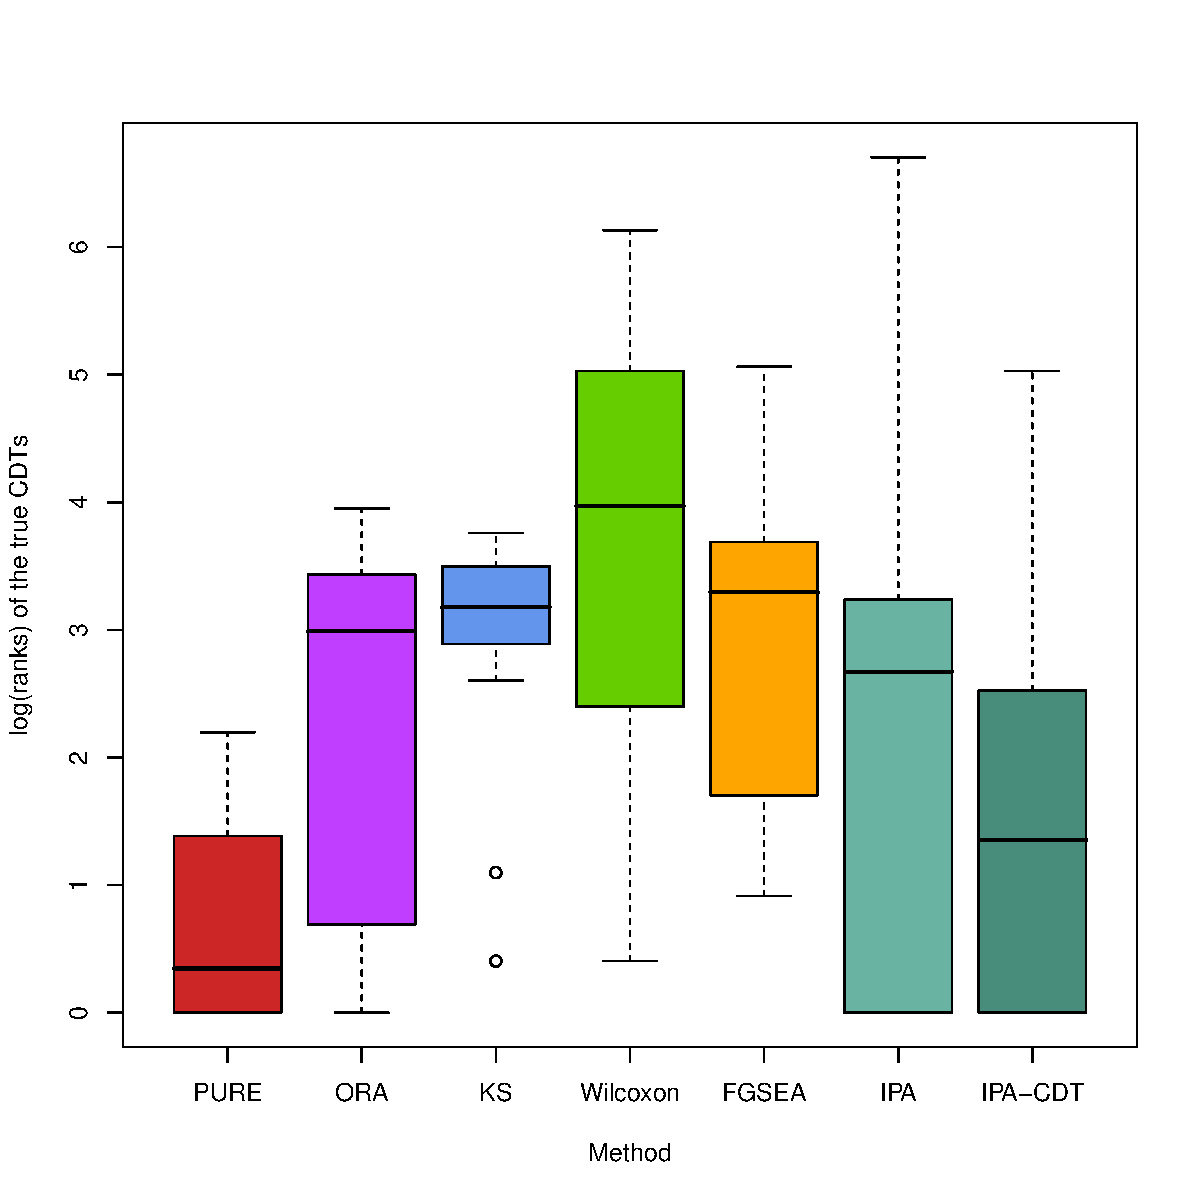
\includegraphics[width=0.49\linewidth]{Figures/RankTarget_vOrg_log.pdf}
%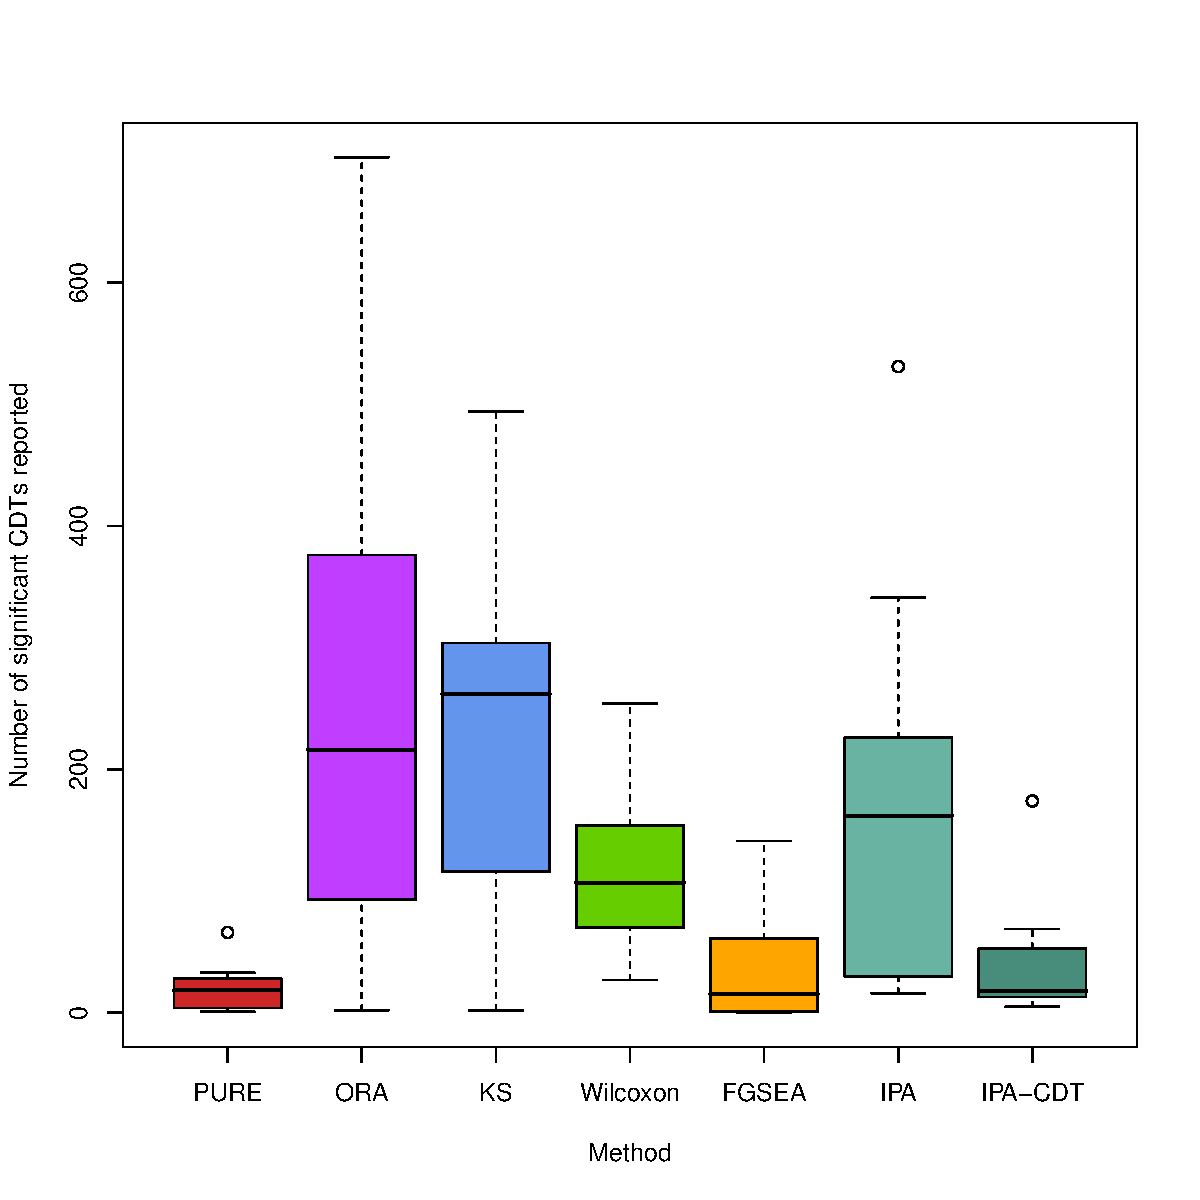
\includegraphics[width=0.49\linewidth]{Figures/NrSigChem_vOrg.pdf}
%%\includegraphics[width=0.32\linewidth]{Figures/pValueTarget_v2.pdf}
%
%\caption{The comparison of PURE and other 5 methods, in term of log(ranks) of true CDTs (left panel) and the number of significant chemicals reported (right panel). In the left panel, a better method would rank the true CDT as low as possible (ideally rank it 1) so lower log(rank) values are better. A CDT that is different from the true CDT and yet reported as significant is a false positive. For this reason, we would like the number of CDTs reported as significant (shown in the right panel) to also be as low as possible. }
%\label{fig:resultFigure}
%\end{center}
%\end{figure*}


\textbf{Definition of success}

To investigate whether the proposed method  is significantly superior to the other methods in term of testing the H1, we would use a Wilcoxon test to compare the ranks and number of CDTs reported by PURE with those provided by the  other methods. 
%The p values for the rank comparison of PURE and IPA-CDT, ORA, KS, FGSEA, IPA, and Wilcoxon are 0.02, 4E-4, 8E-6, 4E-5, 6E-3, and 1E-5, respectively. 
If the rank of the true CDTs is not available in an experiment, we replace the NA ranks by the number of significant CDTs reported in the corresponding experiment plus one, 
e.g. if a method reports a list of 30 significant CDTs but the true CDTs is not included, we assigned 31 to the true CDT's rank.
If the Wilcoxon p value is less than 5\%, we would conclude that the proposed method is statistically better at identifying the causal CDTs than other methods.

Regarding H2, we evaluate the methods' performance based on the same criteria: rank of the target CDT (Methylprednisolone), and the number of CDTs reported. 
%Our proposed method, PURE, is able to identify Methylprednisolone in both experiments with the average rank of 3.25, followed by FGSEA (average = 6.5), ORA (average = 14.75), KS (average = 19.5), Wilcoxon (average = 29), IPA-CDT (average = 393), and IPA (average = 890). Notice that although ORA, KS, Wilcoxon, and FGSEA can identify Methylprednisolone as significant CDT, they cannot determine whether it is present or absent. Also, IPA cannot identify Methylprednisolone in either experiments. More importantly, all other methods, except for FGSEA, reported hundreds of significant CDTs in each experiment, which make it difficult for a researcher to identify a truly effective drug such as Methylprednisolone. Hence, in term of number of CDTs reported, PURE also performs better than other methods. The average number of CDTs reported by PURE is 10 CDTs, whereas that number of FGSEA, IPA-CDT, Wilcoxon, KS, IPA, ORA are 27.5, 103, 189, 216, 238, 553, respectively (Table~\ref{H2Result}). 
Since the sample size is small (only 2 experiments), we do not compute p values for these comparisons. The average of the ranks in these two experiments derived by the benchmarking methods would be directly compared to each other.

\subsection{Discussion}

Beside  benchmarking the studied methods using real data sets as described in previous subsection, in this subsection we  would also compare the differences in theory of our approach versus the other competitive methods.
Moreover, we would discuss how our method improves and addresses the shortcomings of the related methods mentioned in section \ref{chap:ExisingMethodsLimitation} and its differences to other methods in the field. 

Among all the benchmarking methods included in this study, only IPA takes the sign of CDTs - genes associations under consideration and can predict whether a significant CDTs is activated or inhibited (corresponding to H1 and H2), as our proposed method does, so a more detailed theoretical comparison is warranted.
Although IPA derives these two scores  described above for each CDT, the result is solely determined by the z-score: the regulator is determined as ``activated''  or ``inhibited'' if its z-score $\geq 2$ or $\leq -2$, respectively~\cite{kramer2013causal}. In other words, the statistic calculated from the data will determine the outcome. In contrast, our proposed method uses a more classical approach in which the hypotheses are formulated before hand, independently of the data as in a canonical hypothesis testing. Our proposed method  considers each hypothesis separately, and calculates a p-value that will indicate whether the null hypothesis can be rejected. 
For our proposed method, the null hypothesis is that ``CDT X has not had an impact on the measured gene expression changes" whereas the first research hypothesis is that ``CTD X was present and had an impact on the gene expression changes'' and the second, independent, research hypothesis is that ``CTD X was lacking and its absence had an impact on the gene expression changes''. 
The testing done in the proposed approach is more rigorous in terms of statistical testing, but such approach can potentially reject the null hypothesis for both research hypotheses which would be difficult to interpret from a biological perspective. In contrast, the approach used by IPA avoids such potentially ambiguous situations because the z-score can be either positive or negative but not both. The most important difference stemming from these two approaches is that our proposed method  can identify CDTs that can reverse the observed genes expression changes because it considers both sets of statistical hypothesis. This means that our proposed method can be used for drug repurposing - situations in which one is given a   gene expression profile associated with a given disease and the task is to identify a drug that could revert some of the changes. In contrast, IPA only considers the CDTs that are present and focuses whether they are ``activated'' or ``inhibited''. 
Another  difference worth mentioning between IPA and our proposed method  is that while our proposed method  considers and derives a p value corresponding to the hypothesis testing for every CDT in the knowledge base, IPA does not derive z-score for all CDT in the knowledge base. %For example, Methylprednisolone is in the IPA's knowledge base and has z-score in the experiment 15, but no z-score is reported in the experiment 16 (Table ~\ref{H2Result}).

In other cases, the methods using reference gene-expression profiles, such as cMap~\cite{lamb2007connectivity, lamb2006connectivity} , LINCS (http://www.lincscloud.org/l1000/), sscMap~\cite{zhang2009sscmap} or SAM \cite{sirota2011discovery}, compare the gene expression of all genes measured in a disease or drug exposure (called disease's gene signature and drug's gene signature, respectively) to identify pairs of drug-disease that have the opposite signature or pairs of drug-drug that have similar gene signature. The gene signatures are often obtained from few data sets. However, they do not take into consider the fact that insufficient number of data sets to get the gene signatures is problematic. Ein-Dor {et al.} proved  that some gene expression profiles from a same condition are often different and have very few in common~\cite{ein2005outcome}. Our method, on the other hand, only focuses on the given gene profile and would proposes the potential CDT or identify the causal CDT for this specific case. It does not depend on the quantity, quality and lab condition of other experiments used to create the gene signatures database. Moreover, the number of drugs and small-molecule perturbagens in these databases are often limited. For example, in cMAP and SAM, there are less than 200 drugs' signatures. This small amount of drug signature makes this approach impractical. For example, SAM could not identify any potential drug for almost half of the diseases in the database (47 diseases out of 100 diseases). In contrast, our method scans through more than 5,000 CDTs and hence, have more chance to find a potential alternative treatment, especially with new diseases emerging, such as COVID-19. The complexity of comparing all available pairs of drug-disease and drug-drug is $\mathcal{O}(n^2)$ making it cost ineffective on large scale. On the other hand, with a given condition, our methods will derive the result with a complexity of $\mathcal{O}(n)$. One of the biggest drawback of this approach is the limited explanatory power since it cannot interpret which exact genes and mechanisms are affected by the proposed alternative drugs. Our method can identify precisely which and how DE genes are impacted by the proposed drugs.

In comparison with methods that create network of human diseases and potential drugs, our method will provide a list of sorted CDTs according to their p values. One can pick the top few suggested drugs instead of having to verify all the drugs connected to the disease in the disease-drug network. Moreover, our method is also easier to maintain and update regularly since the only source of modification is the CTD database. However, one must re-construct the network of hundred of diseases and drugs once there is any update in the knowledge base.
%
%Our method also utilizes the information of the interactions between drugs and downstream genes, compared to the classical gene set analysis methods.




\clearpage

\section{Conclusion}

In this work, we described the two main approaches that are normally conducted given a gene expression profile: pathway analysis, and upstream analysis.

Given a gene expression profile, pathway analysis can provide the information of which pathways are impacted and the insight of the mechanism activated by the DE genes. We provided a detailed discussion of 2 groups of pathway analysis methods: non-TB and TB methods. We presented some of the most popular tools in each groups and provided guidance for the researchers to choose a suitable method for their analysis. Not only analyzing the methods from theory aspect, we compared the performance some of the most widely used methods on real data sets under three criteria: the ability to identify the truly impacted pathway (the target pathway), the area under the ROC curve using knock-out data sets, and the bias when the null hypothesis is true.

While the ideal pathway analysis method can help one understand the impacted and active pathways, the upstream analysis can actual help us to either identify the cause of the phenotype, and/or identify potential CDTs that is supposed to suppresses the DE genes' expression. 

Here, we propose a causal analysis approach that infers the CDTs responsible for the changes in the gene expression profile, either because their level in the subject's system is higher (hypothesis 1) or lower (hypothesis 2) than normal. 
%This application is a crucial step to treat conditions related to external CDTs since it helps identifying the correct causal CDTs causing observed list of DE genes. 
On one hand,  hypothesis 1 helps identifying the cause of conditions related to external CDTs, and therefore is a crucial step for the treatment process. 
Our proposed method can be applied to time series analysis experiments in which the subjects' gene expression profiles are measured periodically after taking a known medicine. Applying our methods on these profiles would help identify the time point beyond which the effect of the drug ceases to affect the gene expression profiles in a significant way  (e.g. experiments 6-8 in Table \ref{Datasets}).
On the other hand, hypothesis 2 can be interpreted as a prediction of what is lacking in the system but also as a suggestion for a CDT that could reverse the expression changes induced by a disease phenotype, and therefore, is useful in the drug repurposing study. %Recently, a similar approach was applied to the discovery of a treatment for severe cases of COVID-19~\cite{DraghiciCOVID:2021}. 




For validation process, we would used 14 gene expression data sets with different known causal factors and different species for validating the performance of testing H1, and another two data sets for assessment of the ability of testing the H2. %The significance score would show whether our method is more robust than other classical and commercial approaches included in this study, in term of the rank of true CDT, and the number of false positives.

%There are several reasons that limit the accuracy of the existing tools compared to PURE. First, they do not take into consideration the direction of changes in DE genes, i.e., current methods do not take into consideration if a DE gene is up- or down-regulated. Second, they do not utilize the information about CDT-gene interactions as PURE does. Finally, Fisher's exact test may not yield reliable when the number of ``interesting'' genes (i.e. DE genes) is small, which is often the case in gene expression data sets. Instead of DE genes versus total number of  genes, PURE considers the number of interactions supporting (or not)  the testing hypothesis. Because the ratio of edges supporting H1 out of all edges is much higher than the ratio of DE genes out of all available genes in the data sets, PURE is expected produce a significantly more accurate result in more situations.

%\textbf{Limitations}

%\red{Notice that even though Methylprednisolone was proved in a separate clinical trial that it improved the outcome, this finding is arguably not the ground truth because its effectiveness is yet to validate by a big scale clinical study and at the moment it is not the only drug for the COVID-19 treatment. }

%The proposed method, if it works, might be useful in many cases but only as a first -- \emph{computational} -- step to identify potential  causal CDTs (by using  H1), or drugs that could be potentially repurposed (by using H2). As any other type of computational, \textit{in silico} results, anything obtained with this approach will require further validation through laboratory experiments, clinical trials or both.

%The proposed approach, as well as all other methods benchmarked in this study, depend significantly on the quality of the curated chemical-gene expression association database.
%No algorithm would be able to identify the true CDT if no association between this CDT and the DE genes (or any gene) are annotated in the database used.
%Yet, the annotation of the drug-gene association database is the most challenging problem in the field. 
%At any given time, these databases are incomplete, probably partially incorrect, and will evolve as the technology advances and more knowledge is gathered. 
%However, the results shown here, demonstrate the performance of the proposed approach 
%%will yield better results 
%compared to the existing approaches when using currently available resources. 
%The expectation is that an improvement of the quality of the underlying database will improve the results of all methods, rather than favor a particular one. 
%
%Moreover, all CDTs are not equally well studied. CDTs that are more popular and/or widely researched would have more associations with targeted genes discovered than the less popular ones.
%This issue, in turn, could create a potential bias against rare CDTs which would be less likely to be correctly identified.
%The same problem is observed in the pathway analysis field when the pathway analysis methods, including ORA, KS, Wilcoxon, and GSEA, tend to be biased toward small-size pathways~\cite{nguyen2019identifying}.
%
%Another issue with the annotations is that any association can be recorded in the database in two different ways which will also affect the testing hypotheses.
%For example, let us consider a chemical C that increases  the   expression level of a gene G. This can be captured as either ``C increases G'' or, alternatively as ``C deficiency decreases G''. 
%In the experiment in which the chemical C is lacking (data set 14 in Table~\ref{Datasets}), instead of testing the hypothesis 2 that tests whether the chemical C's level is lower than normal, one must test the hypothesis 1 with the true CDT being ``chemical C deficiency''.

%We only benchmark the methods' performance on testing the hypothesis 1. Although hypothesis 2 is extremely useful in the drug repurposing application, it is not included for the following reasons: (i) The hypothesis 1 and 2 are only different in the sign of the interaction, and a method performing well when testing the hypothesis 1 is expected to perform well with the hypothesis 2, as well; (ii) classical gene set methods, namely ORA, KS, Wilcoxon, and FGSEA, just determine whether the CDT is the causal factor the observed expression changes, but cannot distinguish between these two hypotheses; and (iii) lacking some CDTs is sometimes noted in the database with ``CDT deficiency" with reversed signs of the interactions. 
%and (iv) the experiments of chemical deficiency are often complicated, require a lot of clinical trials, take much longer than experiments of hypothesis 1, and they are often not publicly available.
%, and (v) the four classical approaches do not take the types of the interactions between the CDT and genes into consideration and are not able to distinguish the hypothesis 1 and hypothesis 2.

%While benchmarking methods in terms of number of false positives reported, there could be similar CDTs that would have the same effects as the studied CDTs, and therefore, perhaps they should not be counted as false positives. However, in our opinion focusing on the exact chemical that was used to create the phenotype is the most objective and reproducible way for benchmarking the methods.

%Finally, it is important to note that all methods compared here used public annotations from CTD with the exception of IPA which uses Qiagen's proprietary knowledge base. In principle, the fact that IPA's results were less accurate for some of the data sets could be due either to a lower quality underlying knowledge base or to an inferior algorithm. However, this distinction is less important in practical use. A life scientist contemplating the choice of the tools to use in identifying potentially causal CDTs could only consider IPA as a package including both knowledge base and associated algorithm. Therefore, we included the results obtained with IPA, as it is currently available to life scientists. 

%Although this topic is not new, public data sets related to this problem are scarce. To our knowledge, most of the published papers in this field include only one or two data sets in their manuscripts. For example, the causal analysis method in IPA only illustrated their method on two data sets in their manuscript. We considered that insufficient and we strived to use many more data sets. We did an exhaustive search but we only found the 16 data sets that we included here. This is still a small number of data sets but it is an order of magnitude more data sets than used in the articles presenting the existing methods in the field.

\clearpage

% Compile Appendix A
%\phantomsection
%% Create appendix with unnumbered section
\section*{APPENDIX A}

% Add appendix to toc at section level
\addcontentsline{toc}{section}{Appendix A}
\appendix{Stuff and Things}
\label{appendix:stuffAndThings}

My Appendix A...

%\clearpage

%% Compile Appendix B
%\phantomsection
%% Create appendix with unnumbered section
\section*{APPENDIX B}

% Add appendix to toc at section level
\addcontentsline{toc}{section}{Appendix B}
\appendix{More Stuff and Things}
\label{appendix:moreStuffAndThings}

My Appendix B...

%\clearpage
%
%% ...
%
%% Compile Appendix Z
%\phantomsection
%% Create appendix with unnumbered section
\section*{APPENDIX Z}

% Add appendix to toc at section level
\addcontentsline{toc}{section}{Appendix Z}
\appendix{More Stuff and Things, Again}
\label{appendix:moreStuffAndThingsAgain}

My Appendix Z...

%\clearpage

% Compile bibliography
\phantomsection
%% Create references using the unnumbered section formatting
\section*{REFERENCES}

% Add table of contents marker for References
\addcontentsline{toc}{section}{References}

% Add bibliography
%   Replace "bib/mybib" with your directory/bibliography
%\bibliography{/Users/minhnguyen/master} 
\bibliography{/Users/Sorin/Documents/bibliography/master}    %Sorin

% Bibliography style
%   Replace abbrv with whichever style fits your field
%   (https://www.overleaf.com/learn/latex/Bibtex_bibliography_styles)
\bibliographystyle{abbrv}

\section*{REFERENCES}
\bibliographystyle{abbrv}
\addcontentsline{toc}{section}{References}
%\bibliography{/Users/minhnguyen/master/master} 
\bibliography{/Users/minhnguyen/master_v2/master}    %Minh
\clearpage

% Compile abstract
%\phantomsection
%% Use unnumbered section for abstract
\section*{ABSTRACT}

% Add reference to the table of contents {toc} at the section level {section} titled "Abstract" {Abstract}
\addcontentsline{toc}{section}{Abstract}
\centerline{\bf TITLE LINE 1}
\vspace{-0.4cm}
\centerline{\bf TITLE LINE 2 (if needed)}
\vspace{-0.4cm}
\centerline{\bf TITLE LINE 3 (if needed)}

{\setlength\baselineskip{0.3in}
	\begin{center}
	by\\
	\medskip
	{\bf FULL NAME}\\
	\medskip
	{\bf (MONTH YOU WILL GRADUATE) 20XX}\\
	\end{center}
	\Vspc
	\begin{tabular}{ll}
		{\bf Advisor:} & Dr. X \\
		{\bf Major:} & Y \\
		{\bf Degree:} & MASTER OF SCIENCE / MASTER OF ARTS / DOCTOR OF EDUCATION\\
		& / DOCTOR OF PHILOSOPHY
	\end{tabular}
}

\bigskip \bigskip

Your abstract goes here...

%\clearpage

% Compile autobiographical statement
%\phantomsection
%% Create bio section with unnumbered section
\section*{AUTOBIOGRAPHICAL STATEMENT}

% Add reference to the table of contents {toc} at the section level {section} titled "Autobiographical Statement" {Autobiographical Statement}
\addcontentsline{toc}{section}{Autobiographical Statement}
Your bio goes here...


\end{document}
